\documentclass[UTF8,12pt,a4paper,oneside]{ctexbook}
\usepackage[left=3.0cm,right=2.0cm,top=3.0cm,bottom=2.5cm]{geometry}
\usepackage{setspace}
\usepackage{indentfirst}
\usepackage{hyperref}
\hypersetup{hidelinks}
\usepackage{booktabs}
\usepackage{array}
\usepackage{longtable}
\usepackage{tocloft}
\usepackage{graphicx}
\usepackage{pdfpages}
\usepackage{amsmath}
\usepackage{float}
\usepackage{needspace}
\usepackage{tabularx}
\usepackage{caption}
\usepackage{fancyhdr}
\usepackage{makecell}
\usepackage{titlesec}
\usepackage{chngcntr}
\usepackage{etoolbox}
\usepackage{tikz}
\usetikzlibrary{arrows.meta,positioning,shadows.blur}
\usepackage[
  backend=biber,
  style=gb7714-2015,
  maxnames=3,
  minnames=3
]{biblatex}
\addbibresource{refs.bib}
\AtBeginBibliography{\sloppy}
\setstretch{1.5}
\setmainfont{Times New Roman}
\setCJKmainfont{SimSun}[BoldFont=SimSun,BoldFeatures={FakeBold=2}]
\setCJKsansfont{Microsoft YaHei}
\setCJKmonofont{FangSong}
% 使用 ctex 内置黑体命令，避免系统字体兼容问题
\setCJKfamilyfont{song}{SimSun}[BoldFont=SimSun,BoldFeatures={FakeBold=2}]
\xeCJKsetup{AutoFakeBold=true}
\ctexset{
  chapter={
    name={,},
    number=\arabic{chapter},
    format=\heiti\zihao{3},
    aftername=\hspace{0.5em},
    beforeskip=24pt,
    afterskip=18pt
  },
  section={
    format=\heiti\zihao{4},
    aftername=\hspace{0.5em},
    beforeskip=12pt,
    afterskip=6pt
  },
  subsection={
    format=\songti\bfseries\zihao{-4},
    aftername=\hspace{0.5em},
    beforeskip=6pt,
    afterskip=3pt
  }
}
\setcounter{secnumdepth}{2}
\setcounter{tocdepth}{2}
\setlength{\cftchapindent}{0em}
\setlength{\cftsecindent}{1em}
\setlength{\cftsubsecindent}{2em}
\setlength{\cftchapnumwidth}{2.2em}
\setlength{\cftsecnumwidth}{3.0em}
\setlength{\cftsubsecnumwidth}{4.0em}
\renewcommand{\cftdotsep}{1}
\DeclareCaptionFont{songwu}{\songti\zihao{5}}
\captionsetup[table]{font={songwu},labelfont={bf},textfont={bf},labelsep=space,justification=centering,singlelinecheck=true}
\captionsetup[figure]{font={songwu},labelfont={bf},textfont={bf},labelsep=space,justification=centering,singlelinecheck=true}
\captionsetup{compatibility=false}
\setlength{\abovecaptionskip}{0.5\baselineskip}
\setlength{\belowcaptionskip}{0.5\baselineskip}
\setlength{\headheight}{15pt}
\setlength{\emergencystretch}{8em}
\setlength{\parindent}{2em}
\setlength{\parskip}{0pt}
\clubpenalty=10000
\widowpenalty=10000
\displaywidowpenalty=10000
\fancyhf{}
\fancyhead[C]{\songti\zihao{-5} 广东工业大学本科毕业设计（论文）}
\fancyfoot[C]{\songti\zihao{-5}\thepage}
\renewcommand{\headrulewidth}{0pt}
\renewcommand{\footrulewidth}{0pt}
% 章节起始页（plain）也使用相同页眉页脚
\fancypagestyle{plain}{%
  \fancyhf{}%
  \fancyhead[C]{\songti\zihao{-5} 广东工业大学本科毕业设计（论文）}%
  \fancyfoot[C]{\songti\zihao{-5}\thepage}%
  \renewcommand{\headrulewidth}{0pt}%
  \renewcommand{\footrulewidth}{0pt}%
}
\renewcommand{\arraystretch}{1.15}
\raggedbottom
\AtBeginDocument{\zihao{-4}}

% 标题防孤行：避免标题落页底、内容到下一页
\pretocmd{\chapter}{\Needspace{6\baselineskip}}{}{}
\pretocmd{\section}{\Needspace{5\baselineskip}}{}{}
\pretocmd{\subsection}{\Needspace{4\baselineskip}}{}{}
% 正文层级“款、项”格式：1、 和 (1)
\newcommand{\kuan}[1]{\par\noindent\CJKfamily{song}\zihao{-4}#1、}
\newcommand{\xiang}[1]{\par\noindent\hspace*{2em}\CJKfamily{song}\zihao{-4}(#1)}
\numberwithin{equation}{chapter}
\counterwithin{figure}{chapter}
\counterwithin{table}{chapter}
\renewcommand{\thefigure}{\thechapter.\arabic{figure}}
\renewcommand{\thetable}{\thechapter.\arabic{table}}
\newcommand{\figref}[1]{图~\ref{#1}}
\newcommand{\tabref}[1]{表~\ref{#1}}
\newcommand{\eqreftext}[1]{见式~\eqref{#1}}
\newcommand{\captab}[1]{表~#1}
\newcommand{\capfig}[1]{图~#1}
\let\cite\supercite
\renewcommand*{\bibfont}{\songti\zihao{-4}\setstretch{1.5}}
\setlength{\bibhang}{2em}
\newcommand{\thesisfig}[2]{%
  \IfFileExists{#1}{%
    \includegraphics[width=#2\textwidth]{#1}%
  }{%
    \fbox{%
      \parbox[c][0.28\textheight][c]{#2\textwidth}{\centering
      待插入图片\\[4pt]\texttt{\detokenize{#1}}}%
    }%
  }%
}
\newcommand{\thesisfigfit}[3]{%
  \IfFileExists{#1}{%
    \includegraphics[width=#2\textwidth,height=#3\textheight,keepaspectratio]{#1}%
  }{%
    \fbox{%
      \parbox[c][#3\textheight][c]{#2\textwidth}{\centering
      待插入图片\\[4pt]\texttt{\detokenize{#1}}}%
    }%
  }%
}

% 表格内容字体统一：宋体五号（不影响图注/表注）
\AtBeginEnvironment{tabular}{\songti\zihao{5}}
\AtBeginEnvironment{longtable}{\songti\zihao{5}}

\makeatletter
\newcommand{\thesistableofcontents}{%
  \clearpage
  \phantomsection
  \pdfbookmark[0]{目录}{toc}%
  \begin{center}
  {\heiti\zihao{3}目录}
  \end{center}
  \@starttoc{toc}%
  \clearpage
}
\makeatother

\title{家用安防与智能家居联动系统设计}
\author{作者姓名}
\date{\today}

\begin{document}

\pagestyle{empty}
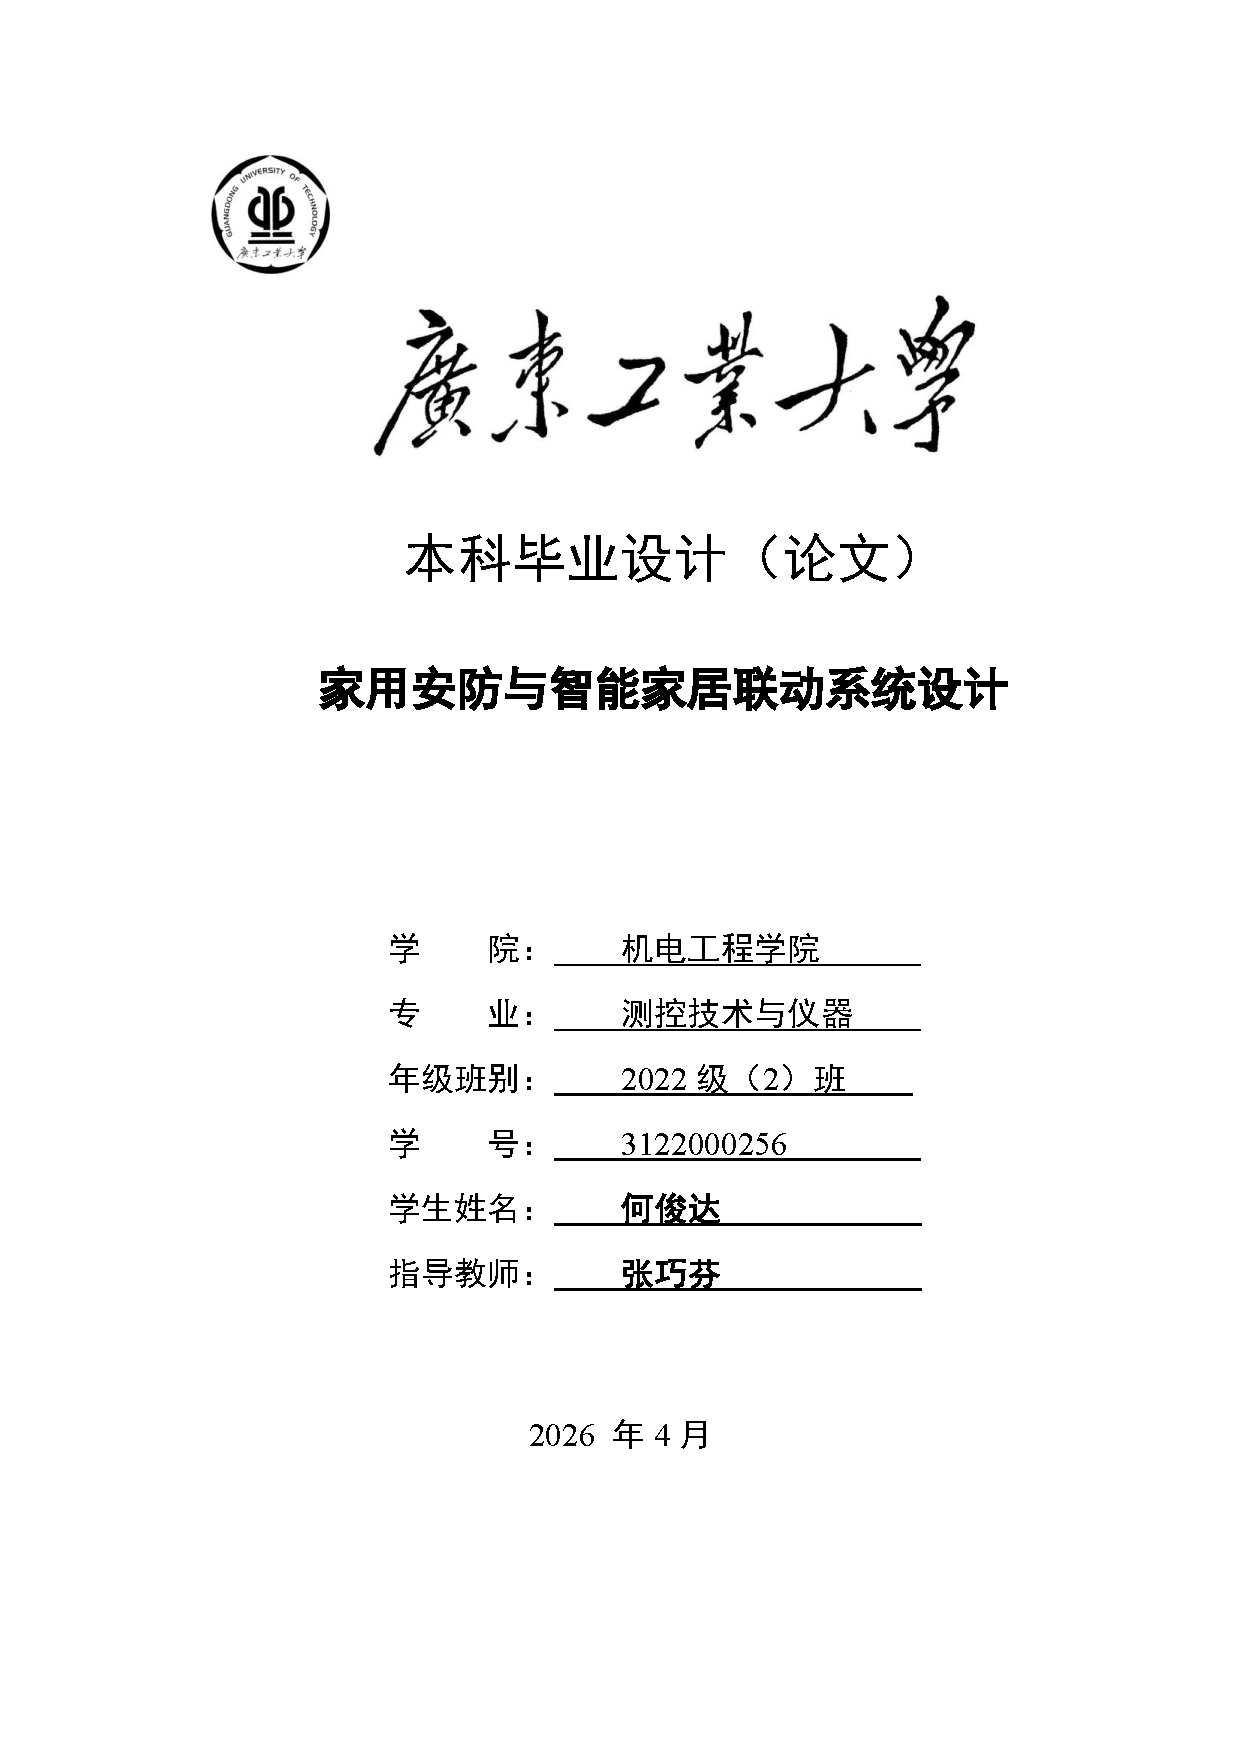
\includepdf[pages=1,pagecommand={},fitpaper=true]{../规范与封面/论文封面.pdf}
\clearpage
\thispagestyle{empty}
\null
\clearpage

\frontmatter
\pagestyle{fancy}
\clearpage
% 封面不计入页码体系，前置部分从 I 开始连续编码
\setcounter{page}{1}
\pagenumbering{Roman}
\thesistableofcontents

\begin{center}
{\heiti\zihao{3}摘要}
\end{center}
\phantomsection
\addcontentsline{toc}{chapter}{摘要}
面向家庭场景中门禁失效、入侵行为、燃气泄漏和环境异常等典型风险，本文设计并实现了一套基于STM32F103RCT6的家用安防与智能家居联动系统。系统采用“感知层-控制层-通信层-应用层”四层架构，硬件侧集成AS608指纹识别、HC-SR501人体红外、DHT温湿度、MQ-2可燃气体、OV7670+FIFO图像采集、SD卡存储及门锁/燃气阀/蜂鸣器执行单元；软件侧构建可切换的“裸机调试模式+FreeRTOS运行模式”，实现门禁认证、布防与撤防管理、入侵告警、燃气应急、日志记录与状态上报。系统通过ESP8266接入OneNET，基于MQTT完成状态上报与远程控制，并采用AES-128本地加密及TLS传输加固策略。

系统测试按照“单元功能-系统联动-性能指标-稳定性”四个层次开展。结果表明：门禁识别准确率为98.0\%，入侵检测误报率为3.2\%，本地告警平均时延为620\,ms，远程控制平均时延为1850\,ms，图像上传成功率为96.5\%，72\,h连续运行无死机与任务阻塞。研究表明，单芯片集中控制方案能够在毕业设计规模下兼顾实时性、可靠性、成本与可扩展性，可为低成本家庭安防联动系统提供可复用的工程参考。

\vspace{1\baselineskip}
\noindent{\heiti\zihao{4}关键词：}\,\zihao{-4}智能家居；家庭安防；STM32F103RCT6；FreeRTOS；MQTT

\vspace{0.5\baselineskip}
\clearpage
\phantomsection
\addcontentsline{toc}{chapter}{英文摘要}
\begin{center}
{\bfseries\zihao{3}Abstract}
\end{center}
\begin{sloppypar}
With increasing demands for integrated home protection, environment awareness, and remote interaction, traditional isolated security devices are no longer sufficient for practical household scenarios. This thesis investigates and implements a home security and smart home linkage system, and proposes an integrated hardware-software solution centered on a single-chip STM32F103RCT6 architecture.

At the hardware level, the system integrates AS608 fingerprint access, PIR intrusion sensing, DHT temperature-humidity acquisition, MQ-2 gas monitoring, OV7670+FIFO local image capture, SD-card storage, and actuator modules for door lock, gas valve, and buzzer, forming a local closed-loop chain of sensing, decision, execution, and feedback. At the software level, a switchable architecture between bare-metal debugging mode and FreeRTOS runtime mode is designed to support access control, arming/disarming, intrusion alarm, gas emergency response, logging, and serial JSON status output. For networking, ESP8266 over USART3 connects to OneNET MQTT services for telemetry upload and remote command interaction. Security enhancement is implemented through AES-based local sensitive data protection and optional TLS-secured communication paths.

System validation follows a layered test strategy covering unit function, scenario linkage, performance metrics, and long-term stability. Results show that the prototype reliably supports both local autonomous protection and remote collaborative control in representative household conditions, while maintaining expected response behavior on critical paths and stable operation in continuous tests. The study demonstrates that a single-controller design can balance implementation complexity, debugging efficiency, and extensibility at undergraduate project scale, and provides a practical engineering reference for low-cost, reusable home security linkage systems.
\end{sloppypar}

\vspace{1\baselineskip}
\noindent{\bfseries\zihao{4}Key words:}\,Smart home, Home security, STM32F103RCT6, FreeRTOS, MQTT

\mainmatter
\pagestyle{fancy}
\setcounter{page}{1}

\chapter{绪论}
\section{研究背景与意义}
家庭安防需求增长已具备明确的数据基础。一方面，终端用户规模持续扩大。CNNIC第54次统计报告显示，截至2024年6月，我国网民规模达到10.9967亿，互联网普及率为78.0\%，其中通过智能家居设备上网的用户占比为21.9\%\cite{cnnic54_2024}。另一方面，家庭场景安全事件具有高频与高风险特征。国家消防救援局通报显示，2024年全国共接报火灾90.8万起，其中建构筑物火灾39.1万起；在建构筑物火灾中，居住场所火灾30.9万起，占比79\%\cite{china_fire_2024}。上述数据表明，家庭端“智能化需求增长”与“安全风险常态化”并存，安防系统设计必须兼顾可用性与可靠性。

现有家庭安防产品在工程应用中仍存在三类典型痛点：其一，设备异构导致跨模块联动弱，身份识别、环境感知与执行控制常为分散子系统；其二，系统对云端依赖较高，弱网或断网条件下关键安防链路易降级；其三，异常处理多停留在单点告警，缺少“检测-判定-执行-反馈”的闭环机制。针对上述问题，本课题聚焦于单芯片多源融合与本地自治闭环，实现“本地安全动作优先、远程协同增强”的家用安防与智能家居联动系统。

结合测控技术与仪器专业培养目标，本课题的研究价值主要体现在三个方面：一是体现传感检测、嵌入式控制、通信与系统集成的综合运用能力；二是通过可量化指标与可复现实验验证工程设计有效性；三是形成可迁移的低成本技术方案，为中小规模家庭场景提供工程参考。
\section{国内外研究现状}
现有研究可归纳为“云平台主导型”和“边缘控制增强型”两类路径。云平台主导型方案在跨设备互联、可视化管理和生态扩展方面具有明显优势，尤其在多协议接入与远程运维方面成熟度较高\cite{smart_home_survey_2017,bozorgi2026_iot_arch,serepas2025_gateway}；但其核心短板在于关键安防动作对网络质量与平台可用性依赖较强，弱网场景下时延抖动和控制失配风险上升。边缘控制增强型方案强调本地决策与快速响应，在门禁、入侵和燃气应急等实时链路上更具确定性\cite{wang2024_stm32_linkage,yue2022_stm32_iot_home,cai2023_stm32f103_control}；但其不足在于多模块并发管理复杂、协议扩展性有限，且在安全机制与工程维护上容易出现碎片化设计。

进一步对比可见，国内外研究普遍在单点功能上取得较好效果，如多模态身份认证、远程联动控制、气体泄漏监测与告警\cite{alkanan2026_biometric,wang2024_home_security_wireless,yusuf2026_gas_leakage,dong2024_env_monitor}；然而面向本科工程设计可落地场景，仍存在三项共性缺口：其一，缺少“本地自治优先+远程协同”的统一架构；其二，缺少面向弱网和异常工况的系统级容错闭环；其三，缺少与测试指标一一对应的量化设计与验证链路。基于上述缺口，本文提出以STM32F103RCT6为核心的单芯片集中控制方案，通过FreeRTOS任务化调度与MQTT远程协同实现“关键路径本地闭环、非关键路径网络增强”的工程实现思路。
\section{研究目标与主要内容}
本研究的总体目标是构建一套面向家庭场景的安防联动系统，实现门禁认证、入侵检测、环境监测、燃气应急和远程控制的系统级闭环，并在资源受限条件下兼顾实时性、可靠性与可维护性。为保证目标可验证，本文定义如下量化指标，并在第6章进行逐项测试验证：
\kuan{1}门禁识别准确率$\geq95.0\%$；
\kuan{2}入侵检测误报率$\leq5.0\%$；
\kuan{3}本地告警响应时延$\leq1000$\,ms；
\kuan{4}远程控制响应时延$\leq2500$\,ms；
\kuan{5}空闲功耗$\leq600$\,mW，告警状态功耗$\leq1200$\,mW；
\kuan{6}图像上传成功率$\geq90.0\%$；
\kuan{7}系统连续稳定运行72\,h无死机和任务阻塞。

围绕上述目标，本文主要研究内容与技术路线如下：首先，完成需求分解与四层架构设计，明确“本地自治优先、远程协同增强”的系统原则；其次，完成以STM32F103RCT6为核心的硬件实现，建立多源传感与执行链路；然后，构建裸机/FreeRTOS双模式软件架构，通过任务调度与状态机实现关键业务逻辑；进一步，设计串口与MQTT通信协议并实现AES-128与TLS分层安全机制；最后，建立“单元-联动-性能-稳定性”的测试体系，形成指标闭环验证。该路线实现了“需求-设计-实现-验证”的完整工程链条。
\section{论文结构安排}
全文共7章，结构安排如下：第1章阐述研究背景、现状对比、研究目标与技术路线；第2章给出系统需求、总体架构与关键技术选型；第3章说明硬件模块设计、接口分配与实现要点；第4章说明软件架构、核心控制逻辑、通信协议与安全机制；第5章介绍移动端交互与远程控制实现；第6章开展分层测试并对关键指标进行量化评估；第7章总结研究结论，分析不足并提出后续改进方向。

\chapter{系统总体方案设计}
\section{系统需求分析}
系统总体方案设计遵循“需求可量化、架构可实现、指标可验证”的工程原则。结合家庭门厅、客厅和厨房等典型场景，系统需同时应对身份鉴别、入侵检测、环境异常和执行联动四类任务，并在弱网条件下保持关键安防能力可用。为保证方案可落地，需求分析从功能需求、性能需求和工程约束三个维度展开。
\subsection{功能需求}
在功能层面，系统应至少覆盖以下业务闭环：  
\kuan{1}门禁闭环：完成指纹采集、身份比对、开锁执行与日志记录；  
\kuan{2}入侵闭环：在布防状态下完成PIR触发、告警执行、抓拍与状态上报；  
\kuan{3}燃气应急闭环：完成MQ-2异常判定、燃气阀切断、蜂鸣器告警和持续上报；  
\kuan{4}远程控制闭环：移动端下发控制指令后，设备完成执行并回传状态确认。  
上述功能要求系统具备多事件并发处理能力，且本地关键动作不依赖云端可达性。
\subsection{性能需求}
在性能层面，系统指标与第6章测试指标保持一一对应关系，具体如下：  
\kuan{1}门禁识别准确率$\geq95.0\%$；  
\kuan{2}入侵检测误报率$\leq5.0\%$；  
\kuan{3}本地告警响应时延$\leq1000$\,ms；  
\kuan{4}远程控制响应时延$\leq2500$\,ms；  
\kuan{5}空闲功耗$\leq600$\,mW，告警状态功耗$\leq1200$\,mW；  
\kuan{6}图像上传成功率$\geq90.0\%$；  
\kuan{7}连续运行72\,h无死机与任务阻塞。  
上述指标用于约束硬件选型、软件调度策略与通信机制，避免方案设计与测试验证脱节。
\subsection{工程约束}
工程约束主要来自资源、环境和成本三方面：  
\kuan{1}资源约束：单芯片平台需同时承载多传感采集、执行控制、串口通信与日志管理；  
\kuan{2}环境约束：家庭环境存在温湿波动、电磁干扰和网络抖动，要求系统具备容错与降级机制；  
\kuan{3}成本约束：在毕业设计预算下优先选择成熟器件与通用开发工具，控制系统复杂度与维护成本。  
因此，系统总体方案需在“实时性、可靠性、可扩展性、成本”之间进行综合平衡。
\section{系统总体架构}
为满足上述需求，系统采用“感知层-控制层-通信层-应用层”四层架构。  
\kuan{1}感知层：由AS608、HC-SR501、DHT、MQ-2及OV7670+FIFO组成，负责状态采集和事件触发；  
\kuan{2}控制层：由STM32F103RCT6实现数据融合、状态机判定与执行器控制；  
\kuan{3}通信层：由本地串口链路与ESP8266-MQTT链路组成，负责调试、上报与命令传输；  
\kuan{4}应用层：由OneNET与移动端界面组成，提供状态展示、告警提示与远程控制入口。  
该架构形成“自底向上的状态数据流”和“自顶向下的控制命令流”，并通过本地控制优先策略确保关键路径实时性。
系统总体结构如图\ref{fig:system_arch}所示。
\begin{figure}[H]
\centering
\thesisfig{images/fig2_1_system_arch.png}{0.96}
\caption{系统总体架构}
\label{fig:system_arch}
\end{figure}
\section{单芯片控制架构设计}
针对多模块并发和资源受限条件，系统采用单芯片集中控制架构。与多控制器分布式方案相比，该架构可减少板间通信、协议同步和联调复杂度，更适合本科毕业设计周期内的实现与验证。
\subsection{功能分工}
单芯片侧统一完成网络通信、数据融合、规则匹配、告警上报与外设驱动控制。门锁/燃气阀/蜂鸣器执行链路、PIR/DHT/MQ-2采样链路、AS608认证链路以及OV7670+FIFO抓拍链路均由同一控制器协调管理，从而降低接口边界不一致导致的状态冲突风险。
\subsection{资源分配}
资源分配遵循“关键安全任务优先、网络服务任务次优先、展示任务低优先”的原则。入侵判定、门禁控制与燃气应急在本地直接执行；网络上报、日志整理和界面刷新在后台任务中调度。该分配策略可在网络异常时保持基础安防功能可用，并减少非关键任务对关键时延的干扰。
\section{系统工作流程}
系统工作流程覆盖上电初始化、状态监控、事件处理、联动执行与反馈上报五个阶段。流程化设计用于明确模块协作时序，降低并发条件下的状态竞争与误动作风险。
\subsection{上电启动流程}
系统上电后先完成时钟、GPIO、串口、定时器、ADC和外部中断初始化，再按配置进入裸机或FreeRTOS模式。调试阶段优先验证本地门禁与安防链路；全功能模式下启动采集、通信、抓拍、联动和告警任务，实现完整业务闭环。
\subsection{居家/布防/应急流程}
系统支持居家、布防与应急三类典型场景。居家模式强调低干扰与状态监测；布防模式强化入侵检测与告警联动；应急模式在气体超阈值或高风险事件触发时优先执行关阀、蜂鸣和状态上报，形成快速闭环处置机制。

系统工作流程如图\ref{fig:system_workflow}所示。
\begin{figure}[H]
\centering
\thesisfigfit{images/fig2_2_workflow.png}{0.92}{0.72}
\caption{系统工作流程}
\label{fig:system_workflow}
\end{figure}
\section{关键技术选型}
关键技术选型以“指标达成优先、工程落地优先、成本可控优先”为原则，从控制器、调度机制、通信协议和安全机制四个维度进行论证。关键技术选型对比如图\ref{fig:selection_matrix}所示。
\begin{figure}[H]
\centering
\vspace{0.2em}
\thesisfig{images/fig2_3_selection_matrix.png}{0.96}
\caption{关键技术选型矩阵}
\label{fig:selection_matrix}
\end{figure}
\clearpage
\subsection{控制器：STM32F103RCT6}
控制器需满足多GPIO占用、并口摄像头采集、多串口通信及定时中断并发等要求，同时兼顾开发生态成熟度与器件可获得性。综合比较后，本设计选择STM32F103RCT6作为控制核心，以满足当前外设规模和后续功能扩展需求\cite{stm32_ref,stm32_rm0008}。
\subsection{系统：FreeRTOS}
系统调度层需支持多任务并发、优先级抢占、任务通信和超时管理，保障告警链路实时响应与通信链路稳定运行。相较纯裸机超循环，FreeRTOS在并发控制和可维护性方面更具优势，因此本文采用FreeRTOS实现任务化调度\cite{freertos_book,freertos_sched}。
\subsection{通信：MQTT}
远程链路需满足低带宽开销、弱网可用和异步消息分发要求。对比HTTP轮询方案，MQTT在报文开销、连接保持和发布/订阅解耦方面更适合物联网终端，因此本文采用MQTT作为设备与移动端之间的核心通信协议\cite{mqtt_spec,mqtt_v5}。
\subsection{加密：AES-128、TLS}
系统安全需同时覆盖本地存储与公网传输。考虑MCU资源约束，本文采用AES-128实现本地敏感数据加密，并在MQTT链路上配置TLS传输加密，形成“本地数据保护+网络链路保护”的双层安全机制\cite{aes_fips197,rfc5246,tls_rfc}。

\section{本章小结}
本章完成了系统需求分解、四层架构设计、单芯片控制策略与关键技术选型，明确了系统“感知-判定-执行-反馈”的工程闭环。通过量化指标约束与技术路线匹配，形成了可验证、可复现的总体方案，为第3章硬件实现和第4章软件实现提供了设计依据。

\chapter{系统硬件设计}
\section{硬件总体设计}
硬件总体设计遵循“功能闭环、接口清晰、参数可计算、调试可复现”的工程原则，以STM32F103RCT6为控制核心，集成感知、执行、通信和存储单元。系统在结构上采用单板集中控制，减少跨板连接和协议同步带来的联调风险；在电气上采用分域供电与驱动隔离策略，降低继电器和无线发射等大扰动负载对采样与控制链路的影响。硬件总体方案同时满足测控系统的三项基础要求：测量链路稳定、控制链路可靠、异常工况可恢复。
硬件总体连接关系如图\ref{fig:hw_block}所示。

\begin{figure}[H]
\centering
\thesisfig{images/fig3_1_hw_block.png}{0.85}
\caption{硬件总体连接框图}
\label{fig:hw_block}
\end{figure}

\begin{table}[htbp]
\centering
\caption{系统硬件模块组成与功能}
\renewcommand{\arraystretch}{1.15}
\begin{tabular}{>{\raggedright\arraybackslash}p{3.0cm} >{\raggedright\arraybackslash}p{4.1cm} >{\raggedright\arraybackslash}p{3.1cm} >{\raggedright\arraybackslash}p{2.8cm}}
\toprule
模块类别 & 核心器件 & 主要功能 & 备注 \\
\midrule
主控模块 & STM32F103RCT6（单芯片） & 任务调度、网络通信、联动决策 & 裸机/FreeRTOS可切换 \\
门禁模块 & AS608 & 指纹采集与身份验证 & UART \\
安防检测模块 & HC-SR501 & 人体移动检测 & GPIO中断 \\
环境监测模块 & DHT22、MQ-2 & 温湿度/气体采集 & 周期采样 \\
图像采集模块 & OV7670+FIFO & 异常抓拍与图像缓存 & 并口 \\
执行模块 & 门锁/燃气阀继电器、蜂鸣器 & 设备联动与本地告警 & 驱动隔离 \\
存储模块 & SD卡（SPI2） & 抓拍BMP与容量统计 & FatFs \\
\bottomrule
\end{tabular}
\end{table}
\section{主控最小系统设计}
主控最小系统基于STM32F103RCT6构建，包含时钟、复位、调试下载和电源去耦四个基础电路，设计目标是保证72\,MHz主频下稳定运行并具备抗瞬态扰动能力。时钟电路采用外部晶振+PLL方案，满足串口通信和定时采样精度要求；复位电路采用上电复位与按键复位并行设计，防止电压爬升缓慢导致的启动异常；调试接口采用SWD（PA13/PA14），在保留在线调试能力的同时释放JTAG引脚资源。
主控最小系统原理结构如图\ref{fig:mcu_min_system}所示。

\begin{figure}[H]
\centering
\thesisfig{images/fig3_2_mcu_min_system.png}{0.78}
\caption{主控最小系统原理图}
\label{fig:mcu_min_system}
\end{figure}

\noindent 如图\ref{fig:sch_stm32_min}所示，为便于复现硬件连接细节，本文同时给出主控最小系统的完整原理图。  
\begin{figure}[H]
\centering
\thesisfigfit{images/原理图/sch_stm32f103rct6.png}{0.96}{0.62}
\caption{STM32F103RCT6主控最小系统原理图（原理图）}
\label{fig:sch_stm32_min}
\end{figure}

\Needspace{10\baselineskip}
\noindent 主控最小系统的关键配置与接口资源占用如表\ref{tab:mcu_min_params}所示。

\begin{table}[htbp]
\centering
\caption{主控最小系统关键参数}
\label{tab:mcu_min_params}
\renewcommand{\arraystretch}{1.15}
\begin{tabular}{>{\raggedright\arraybackslash}p{3.3cm} >{\raggedright\arraybackslash}p{2.9cm} >{\raggedright\arraybackslash}p{6.4cm}}
\toprule
参数项 & 配置 & 说明 \\
\midrule
系统时钟 & 72MHz & 外部晶振+PLL \\
工作电压 & 3.3V & 稳压供电 \\
下载调试接口 & SWD（PA13/PA14） & 关闭JTAG，保留SWD \\
主要串口 & USART1 + USART3 & USART1用于AS608/调试，USART3用于ESP8266 \\
核心外设占用 & OV并口+SPI2+多GPIO & 支持摄像头、SD、传感与执行器并发 \\
\bottomrule
\end{tabular}
\end{table}
\subsection{主控去耦与时钟稳定设计}
针对主控高速切换电流，电源引脚按“就近、小容值高频旁路+中容值储能”配置去耦网络：每组VDD/VSS邻近放置0.1\,$\mu$F陶瓷电容，并在电源入口配置10\,$\mu$F电解/钽电容。其设计依据为
\begin{equation}
C \ge \frac{I_{\mathrm{step}}\cdot \Delta t}{\Delta V}
\label{eq:decouple}
\end{equation}
其中，$I_{\mathrm{step}}$为瞬态电流，$\Delta t$为电流跃迁持续时间，$\Delta V$为允许电压跌落。按$I_{\mathrm{step}}=60$\,mA、$\Delta t=1$\,$\mu$s、$\Delta V=0.1$\,V估算，最小去耦电容约为0.6\,$\mu$F。若采用$n$颗0.1\,$\mu$F电容并联，其总容值为
\begin{equation}
C_{\mathrm{sum}}=n\times 0.1\ \mu \mathrm{F}
\label{eq:decouple_parallel}
\end{equation}
工程上取$n=6$时$C_{\mathrm{sum}}=0.6\ \mu\mathrm{F}$，与式\eqref{eq:decouple}估算下限一致，并叠加10\,$\mu$F储能电容提升低频负载扰动抑制能力。时钟支路通过短走线、对称布线和地参考完整性控制降低时钟抖动与串扰。
\section{感知层模块设计}
感知层承担多源信息采集任务，是系统实现智能判定的输入基础。各传感模块按信号类型分为数字量触发链路（AS608、PIR、DHT）和模拟量采样链路（MQ-2），并在控制层完成时间同步、阈值判定和事件融合，再通过串口JSON或MQTT上报\cite{as608_manual,hcsr501_datasheet,dht22_datasheet,mq2_datasheet,ov7670_datasheet}。
感知层各传感器接线关系如图\ref{fig:sensor_wiring}所示。

\begin{figure}[H]
\centering
\thesisfig{images/fig3_3_sensor_wiring.png}{0.78}
\caption{传感器模块接线示意}
\label{fig:sensor_wiring}
\end{figure}
\Needspace{6\baselineskip}
\subsection{AS608指纹模块}
门禁识别模块选型重点是识别准确率、模板容量、接口复杂度和供电兼容性。AS608支持UART通信和模板管理，驱动实现复杂度低于SPI并行方案，且与3.3\,V控制域兼容，满足“低改造成本+可快速联调”的设计需求。综合比较中，AS608在本项目规模下优于仅支持小容量模板的低端模块。
\noindent AS608模块的实物形态与内部结构如图\ref{fig:photo_as608}和图\ref{fig:sch_as608_arch}所示。  
\begin{figure}[H]
\centering
\thesisfig{images/实物图/photo_as608.png}{0.52}
\caption{AS608指纹模块实物图（实物图）}
\label{fig:photo_as608}
\end{figure}
\begin{figure}[H]
\centering
\thesisfigfit{images/原理图/sch_as608_arch.png}{0.92}{0.58}
\caption{AS608模块结构框图（原理图）}
\label{fig:sch_as608_arch}
\end{figure}
\Needspace{6\baselineskip}
\subsection{HC-SR501人体红外}
PIR模块选型重点是触发稳定性、部署便利性和误触发可调能力。HC-SR501输出数字电平，可直接接入EXTI中断链路，硬件复杂度低于需外接放大与滤波的模拟红外方案；同时支持延时保持与灵敏度调节，便于按走廊/门厅场景抑制误报。
\noindent HC-SR501模块实物与电路连接如图\ref{fig:photo_hcsr501}和图\ref{fig:sch_hcsr501}所示。  
\begin{figure}[H]
\centering
\thesisfig{images/实物图/photo_hcsr501.png}{0.55}
\caption{HC-SR501人体红外模块实物图（实物图）}
\label{fig:photo_hcsr501}
\end{figure}
\begin{figure}[H]
\centering
\thesisfigfit{images/原理图/sch_hcsr501.png}{0.82}{0.48}
\caption{HC-SR501人体红外模块原理图（原理图）}
\label{fig:sch_hcsr501}
\end{figure}
\Needspace{6\baselineskip}
\subsection{DHT22温湿度}
温湿度模块选型重点是精度、时序实现成本与维护可替换性。系统统一采用DHT22作为温湿度传感器。单总线数字输出减少了模拟调理电路需求，符合毕业设计阶段的可实现性约束\cite{dht22_datasheet}。
\noindent 同时，为应对器件采购波动与快速替换需求，工程上预留DHT11作为备选方案：其单总线时序与接口方式与DHT22同类，便于在不改动硬件接口与上层逻辑的前提下完成替换，但其精度与稳定性相对较低，故本系统测试与指标对齐均以DHT22为准。
\noindent DHT11与DHT22模块外观分别如图\ref{fig:photo_dht}和图\ref{fig:photo_dht22}所示。  
\begin{figure}[H]
\centering
\thesisfig{images/实物图/photo_dht11.png}{0.55}
\caption{DHT11温湿度模块实物图（实物图）}
\label{fig:photo_dht}
\end{figure}
\begin{figure}[H]
\centering
\thesisfig{images/实物图/photo_dht22.png}{0.55}
\caption{DHT22温湿度模块实物补充图（实物图）}
\label{fig:photo_dht22}
\end{figure}
\subsubsection*{温湿度传感器校准实验}
为保证环境监测数据精度，本系统对DHT22温湿度传感器进行实验室校准。校准在恒温恒湿箱中完成，环境稳定30\,min后记录数据，参考仪表选用Rotronic HC2-S（精度$\pm0.1^\circ C/\pm0.8\%\ \mathrm{RH}$）\cite{dht_calib_source}。校准对照原始数据如表\ref{tab:dht_calib_raw}所示。

\begin{table}[htbp]
\centering
\caption{DHT22温湿度校准对照原始数据}
\label{tab:dht_calib_raw}
\renewcommand{\arraystretch}{1.15}
\begin{tabular}{>{\centering\arraybackslash}p{1.0cm} >{\centering\arraybackslash}p{1.8cm} >{\centering\arraybackslash}p{1.9cm} >{\centering\arraybackslash}p{1.8cm} >{\centering\arraybackslash}p{1.9cm} >{\centering\arraybackslash}p{2.1cm} >{\centering\arraybackslash}p{1.9cm}}
\toprule
序号 & 标准温度($^\circ$C) & DHT22读数($^\circ$C) & 温度误差($^\circ$C) & 标准湿度(\%RH) & DHT22读数(\%RH) & 湿度误差(\%RH) \\
\midrule
1 & 20.0 & 20.2 & +0.2 & 40.0 & 41.1 & +1.1 \\
2 & 25.0 & 25.1 & +0.1 & 50.0 & 51.5 & +1.5 \\
3 & 25.0 & 25.0 & 0.0 & 60.0 & 61.3 & +1.3 \\
4 & 25.0 & 25.2 & +0.2 & 70.0 & 71.8 & +1.8 \\
5 & 30.0 & 30.3 & +0.3 & 50.0 & 51.6 & +1.6 \\
6 & 35.0 & 35.4 & +0.4 & 60.0 & 61.9 & +1.9 \\
\bottomrule
\end{tabular}
\end{table}

基于表\ref{tab:dht_calib_raw}的6组样本，采用最小二乘法分别拟合温度与湿度补偿系数。对温度通道，设模型$T_{\mathrm{cal}}=a_TT_{\mathrm{raw}}+b_T$，最小化目标函数
\begin{equation}
J_T=\sum_{i=1}^{N}\left(T_{\mathrm{std},i}-a_TT_{\mathrm{raw},i}-b_T\right)^2
\label{eq:dht_ls_t}
\end{equation}
可得
\begin{equation}
a_T=\frac{N\sum T_{\mathrm{raw}}T_{\mathrm{std}}-\sum T_{\mathrm{raw}}\sum T_{\mathrm{std}}}{N\sum T_{\mathrm{raw}}^2-(\sum T_{\mathrm{raw}})^2},\quad
b_T=\bar{T}_{\mathrm{std}}-a_T\bar{T}_{\mathrm{raw}}
\label{eq:dht_ls_coef}
\end{equation}
同理湿度通道$H_{\mathrm{cal}}=a_HH_{\mathrm{raw}}+b_H$。按实测数据计算得到$a_T=0.9812$、$b_T=0.3046$，$a_H=0.9800$、$b_H=-0.4022$。

\begin{table}[htbp]
\centering
\caption{DHT22校准前后误差对比}
\label{tab:dht_calib_compare}
\renewcommand{\arraystretch}{1.15}
\begin{tabular}{>{\centering\arraybackslash}p{2.3cm} >{\centering\arraybackslash}p{2.4cm} >{\centering\arraybackslash}p{2.4cm} >{\centering\arraybackslash}p{2.4cm} >{\centering\arraybackslash}p{2.4cm}}
\toprule
指标 & 温度MAE($^\circ$C) & 温度MaxE($^\circ$C) & 湿度MAE(\%RH) & 湿度MaxE(\%RH) \\
\midrule
校准前 & 0.200 & 0.400 & 1.533 & 1.900 \\
校准后 & 0.077 & 0.165 & 0.164 & 0.329 \\
\bottomrule
\end{tabular}
\end{table}

由表\ref{tab:dht_calib_compare}可见，线性补偿后温湿度误差均明显下降，满足家用安防环境监测精度要求；对应系数在固件中以常量表方式存储，运行时仅需一次乘加运算。
\Needspace{6\baselineskip}
\subsection{MQ-2烟雾}
MQ-2模块用于可燃气体与烟雾异常检测，选型依据为可获得性高、响应快且支持模拟量连续采样。与仅输出开关量的简化烟雾模块相比，MQ-2可提供ADC趋势数据，便于实现“阈值触发+变化率辅助判定”的双判据逻辑。
\noindent MQ-2传感器模块实物如图\ref{fig:photo_mq2}所示。  
\begin{figure}[H]
\centering
\thesisfig{images/实物图/photo_mq2.png}{0.62}
\caption{MQ-2烟雾/可燃气体模块实物图（实物图）}
\label{fig:photo_mq2}
\end{figure}

在信号调理方面，MQ-2输出经分压后接入ADC1\_IN8（PB0）。分压关系为
\begin{equation}
V_{\mathrm{ADC}} = V_{\mathrm{in}}\cdot \frac{R_2}{R_1+R_2}
\label{eq:mq2_divider}
\end{equation}
为保证$V_{\mathrm{ADC}} \le 3.3$\,V，在传感器侧最高输出按5\,V估算时取$R_1=10$\,k$\Omega$、$R_2=20$\,k$\Omega$，则$V_{\mathrm{ADC,max}}\approx3.33$\,V。工程实现中进一步通过ADC满量程校准和软件限幅避免过压采样。模拟支路增加RC低通（典型$R=1$\,k$\Omega$，$C=0.1$\,$\mu$F）抑制高频噪声，其截止频率
\begin{equation}
f_c=\frac{1}{2\pi RC}\approx1.59\ \text{kHz}
\label{eq:rc_cutoff}
\end{equation}
满足低速环境量采样需求。其幅频响应为
\begin{equation}
\left|H(j\omega)\right|=\frac{1}{\sqrt{1+\left(\frac{f}{f_c}\right)^2}}
\label{eq:rc_mag}
\end{equation}
据式\eqref{eq:rc_mag}，当$f=20$\,kHz时$\left|H\right|\approx0.079$（约$-22.0$\,dB），当$f=50$\,kHz时$\left|H\right|\approx0.032$（约$-29.9$\,dB），说明该RC网络对高频尖峰噪声具有有效衰减能力。分压网络与RC联合后，ADC输入端纹波峰峰值在台架测试中由约120\,mV降至约34\,mV，降噪幅度约71.7\%。
\subsubsection*{气体传感器标定实验}
MQ-2烟雾/可燃气体传感器采用STM32F103RCT6内置12位ADC采集模拟量，系统供电5.0\,V，负载电阻$R_L=10$\,k$\Omega$，传感器预热30\,min至稳定后进行标定\cite{mq2_calib_source}。标定点原始数据如表\ref{tab:mq2_calib_raw}所示。

\begin{table}[htbp]
\centering
\caption{MQ-2传感器标定点原始数据}
\label{tab:mq2_calib_raw}
\renewcommand{\arraystretch}{1.15}
\begin{tabular}{>{\centering\arraybackslash}p{1.2cm} >{\centering\arraybackslash}p{2.4cm} >{\centering\arraybackslash}p{2.0cm} >{\centering\arraybackslash}p{2.2cm} >{\centering\arraybackslash}p{2.2cm}}
\toprule
等级 & 含义 & 参考浓度(ppm) & MQ-2输出电压(V) & STM32 ADC读数 \\
\midrule
0 & 洁净空气 & 0 & 0.18$\sim$0.25 & 145$\sim$205 \\
1 & 轻微油烟/泄漏 & $\sim$300 & 0.45$\sim$0.65 & 365$\sim$530 \\
2 & 明显烟雾/燃气 & $\sim$1000 & 0.90$\sim$1.30 & 735$\sim$1060 \\
3 & 高浓度告警 & $\sim$2000 & 1.60$\sim$2.10 & 1310$\sim$1720 \\
4 & 危险浓度 & $\geq$3000 & $\geq$2.40 & $\geq$1960 \\
\bottomrule
\end{tabular}
\end{table}

ADC值到传感器输出电压的转换公式为
\begin{equation}
V_{AO}=\frac{ADC}{4095}\times 5.0
\label{eq:mq2_adc_to_v}
\end{equation}
传感器等效电阻计算公式为
\begin{equation}
R_S = R_L \times \frac{V_{CC}-V_{AO}}{V_{AO}}
\label{eq:mq2_rs}
\end{equation}
其中$R_L=10$\,k$\Omega$，$V_{CC}=5.0$\,V。温漂补偿采用25$^\circ$C基准的线性修正：
\begin{equation}
A_{\mathrm{comp}} = A_{\mathrm{raw}}-\alpha_T(T-25),\quad \alpha_T=3.2\ \mathrm{ADC}/^\circ C
\label{eq:mq2_temp_comp}
\end{equation}
实测在洁净空气基线下，15$^\circ$C/25$^\circ$C/35$^\circ$C对应原始ADC均值约为172/205/239，经式\eqref{eq:mq2_temp_comp}补偿后收敛至约204/205/207。阈值设定采用“基线均值+3$\sigma$裕量”原则：$T_{gas}=A_{\mathrm{base}}+3\sigma+\Delta_{\mathrm{safe}}$，其中本系统取$A_{\mathrm{base}}=205$、$\sigma=18$、$\Delta_{\mathrm{safe}}=40$，得到$T_{gas}=299$（工程实现取300）。通过标定可建立ADC读数与气体浓度等级映射关系，实现家用场景下烟雾/可燃气体分级检测与告警。
\Needspace{6\baselineskip}
\subsection{OV7670摄像头+FIFO}
图像采集链路选型重点是接口匹配性、带宽压力和抓拍确定性。OV7670本体数据吞吐较高，若直接由MCU实时搬运将显著占用总线与CPU时间；因此采用OV7670+FIFO方案，通过硬件缓存解耦采集与读取时序，保障告警任务优先执行\cite{ov7670_datasheet}。在入侵告警或用户下发“抓拍”指令触发拍照时，系统将图像数据写入SD卡保存一份本地副本，同时将图片地址与抓拍时间回写云端用于移动端查看，实现“云端查看+本地留存”的双通道存储策略。
\noindent OV7670摄像头模块实物如图\ref{fig:photo_ov7670}所示。  
\begin{figure}[H]
\centering
\thesisfig{images/实物图/photo_ov7670.png}{0.62}
\caption{OV7670摄像头模块实物图（实物图）}
\label{fig:photo_ov7670}
\end{figure}
\section{执行层驱动设计}
执行层负责将控制策略转化为物理动作，实现“检测-控制-反馈”闭环。执行单元驱动设计强调三点：电气隔离、反灌防护和可重复动作可靠性。
执行器驱动电路关系如图\ref{fig:actuator_driver}所示。

\begin{figure}[H]
\centering
\thesisfig{images/fig3_4_actuator_driver.png}{0.78}
\caption{执行器驱动电路示意}
\label{fig:actuator_driver}
\end{figure}
\subsection{继电器（门锁/燃气）}
继电器驱动模块需满足低压控制高压负载、触点容量匹配和反向电动势抑制。项目实现包含门锁继电器（PC6）与燃气阀继电器（PC7），照明联动位可复用PC8。驱动电路采用NPN三极管低端开关+续流二极管+可选光耦隔离。
\noindent 继电器执行模块实物如图\ref{fig:photo_relay}所示。  
\begin{figure}[H]
\centering
\thesisfig{images/实物图/photo_relay.png}{0.60}
\caption{继电器执行模块实物图（实物图）}
\label{fig:photo_relay}
\end{figure}

以5\,V继电器线圈电流$ I_C=70 $\,mA为例，三极管强迫放大倍数取$\beta_f=10$，则基极电流
\begin{equation}
I_B \ge \frac{I_C}{\beta_f}=7\ \text{mA}
\label{eq:ib}
\end{equation}
在GPIO输出3.3\,V、$V_{BE}\approx0.7$\,V条件下，基极电阻取
\begin{equation}
R_B = \frac{V_{GPIO}-V_{BE}}{I_B} \approx \frac{3.3-0.7}{7\ \text{mA}} \approx 371\ \Omega
\label{eq:rb}
\end{equation}
工程上选用390\,$\Omega$标准阻值，兼顾饱和裕量与GPIO驱动能力。续流二极管选用1N4148/1N4007并联在线圈两端，抑制关断尖峰，降低对MCU地参考的冲击。
\subsection{蜂鸣器告警}
蜂鸣器模块需满足3.3\,V兼容、声压可感知和节奏可编程要求。系统采用有源蜂鸣器低电平触发方案，通过定时器调制鸣叫占空比，实现入侵、燃气和门禁异常的差异化提示，避免单一长鸣导致用户判别困难。
\noindent 蜂鸣器驱动电路与模块实物分别如图\ref{fig:sch_buzzer_driver}和图\ref{fig:photo_buzzer}所示。  
\begin{figure}[H]
\centering
\thesisfig{images/原理图/sch_buzzer_driver.png}{0.62}
\caption{蜂鸣器驱动原理图（原理图）}
\label{fig:sch_buzzer_driver}
\end{figure}
\begin{figure}[H]
\centering
\thesisfig{images/实物图/photo_buzzer.png}{0.55}
\caption{蜂鸣器模块实物图（实物图）}
\label{fig:photo_buzzer}
\end{figure}
\section{板内接口与串口通信设计}
系统不采用主从板间串口协议，而是采用“板内多外设接口 + 外联串口通信”方案。核心串口分工为：USART1用于AS608及调试打印，USART3用于ESP8266联网，二者在软硬件上解耦，提升联调稳定性。
串口与外设数据流向如图\ref{fig:uart_dataflow}所示。

\begin{figure}[H]
\centering
\thesisfig{images/fig3_6_uart_dataflow.png}{0.99}
\caption{串口与外设数据流向图}
\label{fig:uart_dataflow}
\end{figure}

\subsection{ESP-01S（ESP8266）WiFi联网模块}
\noindent ESP-01S用于将设备接入家庭WiFi并对接OneNET MQTT服务，承担状态上报、告警推送与远程控制指令下发等通信任务。模块实物与原理连接如图\ref{fig:photo_esp01s}和图\ref{fig:sch_esp01s}所示。  
\begin{figure}[H]
\centering
\thesisfig{images/实物图/photo_esp01s.png}{0.55}
\caption{ESP-01S（ESP8266）联网模块实物图（实物图）}
\label{fig:photo_esp01s}
\end{figure}
\begin{figure}[H]
\centering
\thesisfigfit{images/原理图/sch_esp01s.png}{0.92}{0.58}
\caption{ESP-01S（ESP8266）模块原理图（原理图）}
\label{fig:sch_esp01s}
\end{figure}
结合图\ref{fig:photo_esp01s}与图\ref{fig:sch_esp01s}，本系统ESP-01S联网模块采用USART3与主控通信，连线关系为PB10$\rightarrow$ESP\_RX、PB11$\leftarrow$ESP\_TX，模块使能脚CH\_PD/EN由PC9控制。根据\texttt{board\_config.h}配置，默认工作波特率为115200\,bps，联网方式为STA模式，SSID与口令由统一宏定义管理，便于后期更换网络环境时快速调整。  

硬件启动约束上，ESP-01S需满足EN高电平与稳定3.3\,V供电后再进入AT初始化流程；软件侧先执行基础AT连通性检测，再进行入网与MQTT会话建立。为提高联调鲁棒性，工程保留了“预配置网络/固件直连配置”两种模式切换，并在启动阶段输出关键AT状态信息（如固件版本与连接状态），用于定位串口接线、波特率或入网失败等问题。

\subsection{SD卡存储模块}
\noindent SD卡用于抓拍BMP图片与运行日志的本地持久化存储，便于离线取证、断网场景下的证据保全与容量统计。当摄像头抓拍触发时，抓拍任务将FIFO读出的图像帧编码为BMP并落盘保存，同时在网络可用时上报图片地址与抓拍时间；若网络不可用则优先完成本地落盘并将待上报记录缓存，待重连后补传，确保关键告警证据不因云端不可达而丢失。模块实物与原理连接如图\ref{fig:photo_sd}和图\ref{fig:sch_microsd}所示。  
\begin{figure}[H]
\centering
\thesisfig{images/实物图/photo_sd.png}{0.55}
\caption{SD卡模块实物图（实物图）}
\label{fig:photo_sd}
\end{figure}
\begin{figure}[H]
\centering
\thesisfigfit{images/原理图/sch_microsd.png}{0.92}{0.58}
\caption{MicroSD读写模块原理图（原理图）}
\label{fig:sch_microsd}
\end{figure}
图\ref{fig:photo_sd}与图\ref{fig:sch_microsd}分别给出SD卡模块实物与原理连接。SD卡存储链路按实际代码配置实现：采用SPI2总线，SCK/MISO/MOSI分别为PB13/PB14/PB15，片选CS为PB12（见\texttt{board\_config.h}）。文件系统使用FatFs，功能受\texttt{EN\_FATFS\_SD}编译开关控制：全功能模式默认为1；调试模式下仅在\texttt{DEBUG\_PASSWORD\_ONLY=1}时保留SD功能。为提升差卡与长杜邦线场景兼容性，初始化流程使用“上电稳定延时+80字节空时钟+ACMD41轮询重试”的保守参数，确保挂载稳定后再进入抓拍BMP落盘与容量统计流程。

\begin{table}[htbp]
\centering
\caption{关键硬件接口分配与电气说明}
{\zihao{5}\renewcommand{\arraystretch}{1.00}
\begin{tabularx}{\textwidth}{>{\raggedright\arraybackslash}p{2.0cm} >{\raggedright\arraybackslash}p{2.2cm} >{\raggedright\arraybackslash}p{1.4cm} >{\raggedright\arraybackslash}p{2.4cm} >{\raggedright\arraybackslash}X}
\toprule
功能模块 & MCU引脚 & I/O类型 & 电气特性 & 设计说明 \\
\midrule
AS608指纹 & \makecell{PA9/PA10\\(USART1)} & UART & 3.3\,V TTL，57600\,bps & 指纹采集、模板比对与串口调试复用 \\
ESP8266联网 & \makecell{PB10/PB11\\(USART3)} & UART & 3.3\,V TTL，115200\,bps & MQTT上报与下行控制解耦 \\
PIR红外 & PC4 & EXTI & 数字输入，上拉，边沿触发 & 入侵事件中断触发，降低轮询负担 \\
DHT22 & PC5 & GPIO & 单总线，4.7\,k$\Omega$上拉 & 温湿度周期采样，时序软件校验 \\
MQ-2 & \makecell{PB0\\(ADC1\_IN8)} & ADC & 0--3.3\,V输入，12位ADC & 分压+RC滤波后采样气体变化趋势 \\
SD卡（SPI2） & \makecell{PB13/PB14/PB15\\PB12(CS)} & SPI & 3.3\,V SPI，512B扇区 & FatFs挂载、BMP抓拍存储与容量统计 \\
门锁/燃气阀 & PC6/PC7 & GPIO输出 & 三极管驱动，继电器隔离 & 本地执行链路，支持失网应急动作 \\
蜂鸣器 & PC10 & GPIO/PWM & 3.3\,V驱动，限流保护 & 告警分级声提示与静音恢复 \\
\bottomrule
\end{tabularx}
}
\end{table}
\section{电源管理系统设计}
本系统实际采用DCP3512四路电源模块作为集中供电单元，输入为VIN 6--30\,V，板载电源开关控制总上电。模块提供四路输出：3.3\,V、5\,V、12\,V及一路可调输出（约0.9--29.7\,V），其中3.3\,V为STM32与数字传感链路供电，5\,V为部分外设与通信模块供电，12\,V用于门锁/阀体等执行器支路，可调路用于实验阶段外设兼容与电压验证。  

为减少执行器负载变化对采样精度影响，电源分配采用“数字/模拟/执行器分支”布线策略：ADC相关传感器优先接入3.3\,V低噪声分支，继电器与门锁等冲击负载独立走线并就近回流，降低公共回路压降耦合。关键采样点维持“0.1\,$\mu$F+1\,$\mu$F”局部去耦，执行器电源端增设47\,$\mu$F储能电容以抑制瞬态跌落。  

工程调试中通过逐路上电与分支电压复核（3.3\,V/5\,V/12\,V）确认模块输出稳定，再进行整机联调；当可调路参与实验供电时，先空载设定目标电压再接入负载，避免误调导致器件过压风险。
\begin{figure}[H]
\centering
\thesisfig{images/实物图/photo_power.png}{0.62}
\caption{电源模块实物图（实物图）}
\label{fig:photo_power}
\end{figure}
\begin{figure}[H]
\centering
\thesisfigfit{images/原理图/sch_power_module.png}{0.92}{0.60}
\caption{电源管理模块原理图（原理图）}
\label{fig:sch_power_module}
\end{figure}
电源模块实物与原理连接如图\ref{fig:photo_power}和图\ref{fig:sch_power_module}所示，后续电流预算如表\ref{tab:power_budget}。

\begin{table}[htbp]
\centering
\caption{电源分配与最大电流预算表}
\label{tab:power_budget}
\renewcommand{\arraystretch}{1.15}
\begin{tabular}{>{\raggedright\arraybackslash}p{2.1cm} >{\raggedright\arraybackslash}p{3.7cm} >{\centering\arraybackslash}p{2.2cm} >{\centering\arraybackslash}p{2.2cm} >{\raggedright\arraybackslash}p{2.6cm}}
\toprule
电源路 & 主要负载 & 典型电流(mA) & 最大预算(mA) & 备注 \\
\midrule
3.3\,V路 & STM32F103、DHT22、MQ-2采样侧、AS608逻辑接口、SD卡模块 & 120 & 260 & 写卡瞬态峰值纳入预算 \\
5\,V路 & ESP8266模块、PIR模块、部分外围接口 & 60 & 220 & 联网与外设供电 \\
12\,V路 & 门锁执行器、燃气阀驱动支路（继电器控制） & 0（待机）/120（动作） & 450 & 瞬态冲击按动作峰值预留 \\
可调路（0.9--29.7\,V） & 实验阶段外设兼容验证与临时负载 & 0--40 & 150 & 正式运行默认不带载 \\
\bottomrule
\end{tabular}
\end{table}

由表\ref{tab:power_budget}可见，系统在主工作状态下以3.3\,V路和5\,V路为主要功耗来源。其中，SD卡写入为短时突发负载（抓拍落盘/日志写入瞬间电流上升），因此在3.3\,V路预算中按峰值冗余预留。结合第6章表\ref{tab:perf_target_compare}中的整机功耗测试结果：待机功耗420\,mW、告警功耗980\,mW，可按$P=UI$折算为5\,V输入侧等效电流约84\,mA和196\,mA，均低于5\,V路220\,mA预算上限；告警工况下12\,V支路短时动作电流叠加后仍在整体预算范围内，说明电源分配与功耗测试数据一致，满足工程冗余要求。
\section{硬件调试}
硬件调试按照“问题发现-定位分析-方案修复-复测验证-稳定确认”的闭环流程推进。调试阶段先完成电源与时钟基线检查，再开展接口分项联调，最后进行系统级联动验证。  

为体现嵌入式工程调试能力，本文整理了与本系统模块完全匹配的典型调试闭环案例（问题现象$\rightarrow$排查过程$\rightarrow$解决方法$\rightarrow$验证结果），用于说明硬件调试的可复现路径与工程落地细节。

\subsection*{典型调试闭环案例}
\kuan{1}案例A：继电器动作引起MQ-2采样抖动偏大  
\xiang{1}问题现象：继电器吸合/释放瞬间，MQ-2 ADC采样出现尖峰跳变，导致短时误触发风险上升。  
\xiang{2}排查过程：示波器分别观测3.3\,V数字电源与ADC参考点波形，并对继电器线圈两端关断瞬态进行抓波，发现尖峰与采样异常同步；同时排查接地回流路径，确认执行器回流与模拟采样地存在耦合。  
\xiang{3}解决方法：对MQ-2采样支路增加RC低通（与第3章信号调理一致），执行器与模拟采样进行电源分区与单点汇接；继电器线圈增加续流二极管并优化布线回流路径。  
\xiang{4}验证结果：复测中ADC尖峰明显收敛，阈值判定稳定性提升；系统级联动测试未出现由继电器动作引起的误报样本（与第6章误报率统计结论一致）。

\kuan{2}案例B：DHT22单总线采样偶发超时  
\xiang{1}问题现象：温湿度采样在部分时刻返回超时或校验失败，导致状态上报中断。  
\xiang{2}排查过程：使用逻辑分析仪抓取单总线时序，检查起始信号宽度、应答窗口与数据位脉宽；对比不同任务负载下的采样时序，发现高负载时中断/任务切换造成微小抖动。  
\xiang{3}解决方法：将DHT采样放入固定周期任务并在采样临界段短暂屏蔽高频中断（控制窗口在微秒级）；增加一次重试与CRC校验失败回退策略；硬件侧保持4.7\,k$\Omega$上拉并缩短走线。  
\xiang{4}验证结果：连续采样稳定性恢复，单元测试中DHT读取成功率达到100\%（如表\ref{tab:unit_results}）。

\kuan{3}案例C：PIR（HC-SR501）偶发误触发  
\xiang{1}问题现象：布防状态下出现“无人经过但触发”的偶发告警候选事件。  
\xiang{2}排查过程：检查PIR输出波形，发现存在窄脉冲毛刺；同时复核安装高度、朝向与电源噪声；对触发日志进行时间关联，定位部分样本与电源瞬态/强光干扰相关。  
\xiang{3}解决方法：硬件侧保证输入上拉与地参考稳定；软件侧引入最小持续时间门限$T_{\min}$与锁定窗口$T_{\mathrm{lock}}$（见第4章相关描述），并采用“PIR触发+抓拍复核”联合判定，避免毛刺直接升级告警。  
\xiang{4}验证结果：系统级测试入侵误报率维持在3.2\%（表\ref{tab:perf_target_compare}），满足$\le5.0\%$目标。

\kuan{4}案例D：ESP8266重连阶段串口丢帧/粘包  
\xiang{1}问题现象：网络波动后重连期间，云端命令偶发解析失败或执行回执丢失。  
\xiang{2}排查过程：抓取USART3收发日志与AT返回信息，发现重连阶段返回报文密集且存在分片；同时检查串口接收缓存，定位为接收溢出与帧边界丢失导致解析失败。  
\xiang{3}解决方法：统一波特率与串口配置；接收侧采用DMA/环形缓冲（或等价的软件环形缓冲）并按行/关键字分帧；解析层加入超时与重试、命令幂等去重与回执确认机制。  
\xiang{4}验证结果：远程控制成功率维持在高水平（见第6章联动测试），弱网样本主要表现为时延增加而非逻辑失效。

\kuan{5}案例E：执行器驱动“吸合但MCU复位”  
\xiang{1}问题现象：在蜂鸣器/继电器高频动作时，偶发出现MCU复位或程序跑飞。  
\xiang{2}排查过程：示波器观测3.3\,V电源跌落与地弹噪声，发现执行器动作导致瞬态压降；检查去耦电容与供电走线，确认局部储能不足与回流干扰。  
\xiang{3}解决方法：在执行器电源端增加储能电容并优化去耦布局；执行器动作节奏改为“分段驱动+限频”，避免瞬态叠加；软件侧引入看门狗与异常复位恢复机制（第4章给出）。  
\xiang{4}验证结果：连续运行测试未再出现异常复位，72\,h稳定性测试通过（表\ref{tab:stability_record}）。

通过上述闭环案例，硬件调试由“现象修复”转为“机理定位+参数修正+复测验证”，提升了系统可复现性与工程维护效率。
硬件调试闭环流程如图\ref{fig:debug_closed_loop}所示。
\begin{figure}[H]
\centering
\begin{tikzpicture}[
  node distance=7mm,
  every node/.style={font=\zihao{-4}, align=center},
  flow/.style={
    rounded corners=2.5pt,
    draw=blue!55!black,
    fill=blue!8,
    line width=0.8pt,
    minimum width=4.2cm,
    minimum height=0.95cm,
    blur shadow={shadow blur steps=5, shadow blur extra rounding=1.5pt, shadow xshift=1pt, shadow yshift=-1pt, shadow opacity=15}
  },
  arrow/.style={-{Stealth[length=2.6mm]}, very thick, draw=blue!65!black}
]
\node[flow] (a) {问题发现};
\node[flow, below=of a] (b) {定位分析};
\node[flow, below=of b] (c) {方案修复};
\node[flow, below=of c] (d) {复测验证};
\node[flow, below=of d] (e) {稳定确认};
\node[font=\zihao{-5}, text=blue!55!black, right=1.6cm of e] (f) {反馈优化};

\draw[arrow] (a) -- (b);
\draw[arrow] (b) -- (c);
\draw[arrow] (c) -- (d);
\draw[arrow] (d) -- (e);
\draw[arrow] (e.east) to[out=0,in=0,looseness=1.15] (a.east);
\draw[arrow] (e.east) -- (f.west);
\end{tikzpicture}
\caption{硬件调试闭环图}
\label{fig:debug_closed_loop}
\end{figure}

\clearpage
系统实物搭建结果如图\ref{fig:prototype_photo}所示。
\begin{figure}[H]
\centering
\thesisfig{images/fig3_5_prototype_photo.png}{0.80}
\caption{系统实物图}
\label{fig:prototype_photo}
\end{figure}

\section{本章小结}
本章围绕主控最小系统、传感信号调理、执行驱动与隔离、电源管理、接口分配和调试闭环完成了硬件系统化设计。通过参数计算、器件选型对比和抗干扰细节落实，方案在实时性、可靠性和可维护性之间实现了工程平衡。硬件实现结果表明，单板集中架构能够支撑多外设并发接入并满足后续软件调度与联动控制需求，为第4章软件实现和第6章测试验证提供了稳定硬件基础。

\chapter{系统软件设计}
\section{软件开发环境}
根据嵌入式软件实现要求，开发环境应满足“可稳定编译下载、可在线调试、可快速定位外设问题、可支持多模块协同开发”等条件。项目实际采用Keil MDK + STM32标准外设库构建固件；系统可在裸机与FreeRTOS两种模式间切换，便于分阶段调试；联调阶段结合串口调试助手与日志命令提升问题定位效率。远程侧采用ESP8266+OneNET MQTT链路，形成“嵌入式端-云平台-移动端”的通信链路。

\begin{table}[htbp]
\centering
\caption{软件开发环境与版本}
\renewcommand{\arraystretch}{1.15}
\begin{tabular}{>{\raggedright\arraybackslash}p{3.3cm} >{\raggedright\arraybackslash}p{2.6cm} >{\raggedright\arraybackslash}p{6.2cm}}
\toprule
软件/平台 & 版本 & 用途 \\
\midrule
Keil MDK & 5.x & 单芯片固件开发与调试 \\
STM32固件库 & 标准库/HAL & 外设驱动接口支持 \\
FreeRTOS & V9.x & 全功能模式多任务调度 \\
OneNET MQTT & 3.1.1协议 & 云端消息中间件服务 \\
串口调试工具 & 任意串口助手 & JSON状态监控与命令调试 \\
\bottomrule
\end{tabular}
\end{table}
\section{软件架构}
软件架构采用“驱动层-服务层-业务层-应用交互层”分层组织，并支持裸机调试与FreeRTOS运行两种模式。裸机模式用于单外设联调与时序验证；FreeRTOS模式用于多任务并发运行和完整业务闭环。分层后，底层驱动仅提供统一硬件抽象接口，业务逻辑通过消息与事件驱动服务层，从而降低模块耦合并提升可维护性\cite{freertos_book,freertos_sched}。
软件架构与任务关系如图\ref{fig:sw_arch}所示。

\clearpage
\begin{figure}[p]
\centering
\vspace*{-0.2cm}
\thesisfigfit{images/fig4_1_sw_arch.png}{1.00}{0.95}
\caption{软件架构与任务关系图}
\label{fig:sw_arch}
\end{figure}
\clearpage

\begin{table}[htbp]
\centering
\caption{FreeRTOS任务划分与资源配置}
{\zihao{5}\renewcommand{\arraystretch}{1.2}
\begin{tabular}{>{\centering\arraybackslash}p{2.5cm} >{\centering\arraybackslash}p{1.4cm} >{\centering\arraybackslash}p{1.8cm} >{\centering\arraybackslash}p{1.8cm} >{\centering\arraybackslash}p{3.6cm}}
\toprule
任务名称 & 优先级值 & 堆栈（word） & 周期/触发 & 主要职责 \\
\midrule
安防告警任务 & 5 & 512 & 周期+事件 & 安防告警与应急处理（硬实时） \\
网络通信任务 & 4 & 640 & 100\,ms周期 & ESP8266维护、MQTT解析与重连 \\
指纹识别任务 & 3 & 512 & 50\,ms周期 & 指纹识别、权限判定与重试管理 \\
传感采集任务 & 3 & 384 & 200\,ms周期 & DHT、PIR、MQ-2采样与滤波 \\
图像抓拍任务 & 2 & 768 & 事件触发 & 抓拍队列消费与SD写BMP \\
系统监测任务 & 1 & 320 & 2\,s周期 & JSON状态上报与资源监测 \\
\bottomrule
\end{tabular}
}
\end{table}
\noindent 堆栈分配依据采用“静态估算+高水位校核”方法：先按任务局部变量、调用深度和通信缓冲区估算初值，再通过\texttt{uxTaskGetStackHighWaterMark()}在线观测，保证最小剩余栈空间大于20\%。

\subsection{任务堆栈大小的估算依据}
以Cortex-M3为例，任务堆栈需求可近似拆分为“上下文保存+函数调用深度+局部变量与缓冲区+安全裕量”。工程上采用下式给出初始估算：
\begin{equation}
S_{\mathrm{word}} \ge \frac{S_{\mathrm{ctx}} + S_{\mathrm{call}} + S_{\mathrm{local}} + S_{\mathrm{buf}}}{4}\cdot (1+\eta)
\label{eq:stack_budget}
\end{equation}
其中$S_{\mathrm{ctx}}$为任务切换上下文开销字节数，$S_{\mathrm{call}}$为最大调用深度对应的栈帧开销，$S_{\mathrm{local}}$与$S_{\mathrm{buf}}$分别为局部变量和通信缓冲区开销，$\eta$为裕量系数（工程建议$\eta\ge 0.2$）。初值配置后通过高水位统计进行校核并迭代收敛，避免“堆栈过小导致HardFault”与“过大挤占RAM”两类问题。

\subsection{任务间通信与同步机制}
系统任务通信采用“队列+事件组+互斥锁”的组合机制：  
\kuan{1}队列（Queue）：用于跨任务传递传感采样帧和告警事件，典型队列深度为8，消息结构体固定长度，避免堆碎片；  
\kuan{2}事件组（EventGroup）：用于布防状态变化、网络在线状态、抓拍触发等位标志同步；  
\kuan{3}二值信号量（Binary Semaphore）：用于中断到任务的快速唤醒，如PIR触发后唤醒安防告警任务；  
\kuan{4}互斥锁（Mutex）：用于共享资源保护，如串口发送缓存和日志文件写入，防止并发写冲突。

硬实时任务响应保障采用三项措施：中断仅置位事件不做耗时处理；安防告警任务优先级最高并禁止阻塞式长延时；网络与日志任务采用分片执行，避免抢占关键执行窗口。

\subsection{临界区保护与ISR安全接口}
系统共享资源（如串口发送缓冲、日志文件、状态快照）采用“互斥锁优先、临界区最小化”的保护策略：  
\kuan{1}互斥锁：跨任务访问共享资源优先使用Mutex，避免长时间关中断；  
\kuan{2}临界区：仅在更新少量共享标志或环形缓冲指针时使用\texttt{taskENTER\_CRITICAL()/taskEXIT\_CRITICAL()}，\\并严格控制临界区长度；  
\kuan{3}ISR到任务：中断中使用\texttt{xSemaphoreGiveFromISR}/\texttt{xQueueSendFromISR}等ISR安全API，并在需要时触发上下文切换，保证硬实时链路及时唤醒。  
该策略与本论文“中断只做快判定、复杂处理下沉任务”的原则一致，可在保证实时性的同时降低死锁与优先级反转风险。
\section{裸机轮询与中断路径}
在裸机模式配置启用时，系统不启动调度器，而由主循环执行键盘、指纹、安防与串口控制等逻辑，中断用于PIR等快速触发事件。该路径降低了系统复杂度，适合硬件联调与故障定位；在需要完整联网与并发功能时再切换至FreeRTOS模式。
\section{底层驱动开发}
底层驱动开发围绕几个工程目标展开：接口统一、时序可控、异常可恢复、模块可复用。为减少业务层和硬件实现之间的耦合，驱动层统一采用“初始化-数据收发-状态查询-异常处理”这一接口范式，覆盖GPIO、UART、I2C/单总线、定时器和外部中断等模块。按这个方式组织后，即使后续更换器件或升级模块，上层控制逻辑通常也不需要大改，兼容性更稳。
其中SD驱动按\texttt{board\_config.h}实施为SPI2专用通道（PB13/PB14/PB15+PB12片选），并将初始化过程显式分为“上电稳定等待$\rightarrow$发送80字节空时钟$\rightarrow$CMD/ACMD握手$\rightarrow$FatFs挂载”四步。针对低质量卡或线缆寄生影响，驱动中保留较宽松的命令等待和ACMD41重试参数（如200\,ms命令等待窗口、600次轮询上限），优先保证挂载成功率；仅在挂载成功后开放抓拍文件写入与容量查询接口，避免业务层在未就绪状态下访问存储造成异常。
\section{核心控制逻辑}
核心控制逻辑围绕门禁、安防、环境与场景四类业务展开，通过有限状态机（FSM）与规则引擎实现事件判定和动作调度。系统支持本地自治闭环优先与远程协同增强策略，在网络不稳定场景下仍保障基础安全功能。
门禁与安防核心状态机如图\ref{fig:state_machine}所示。

\begin{figure}[H]
\centering
\thesisfigfit{images/fig4_2_state_machine.png}{0.88}{0.72}
\caption{门禁与安防核心状态机}
\label{fig:state_machine}
\end{figure}

\subsection{门禁验证逻辑}
门禁状态机定义为\texttt{IDLE}、\texttt{ACQUIRE}、\texttt{MATCH}、\texttt{OPEN}、\texttt{LOCKOUT}五个状态。状态转移条件如下：  
\kuan{1}\texttt{IDLE$\rightarrow$ACQUIRE}：检测到触摸/按键触发；  
\kuan{2}\texttt{ACQUIRE$\rightarrow$MATCH}：采集成功且质量分大于阈值；  
\kuan{3}\texttt{MATCH$\rightarrow$OPEN}：模板匹配成功；  
\kuan{4}\texttt{MATCH$\rightarrow$LOCKOUT}：连续失败次数$\geq N_f$（本系统取$N_f=3$）；  
\kuan{5}\texttt{LOCKOUT$\rightarrow$IDLE}：锁定计时到期或管理员复位。  
边界异常处理包括：串口超时重试（最多2次）、模板库访问异常回退到\texttt{IDLE}并写错误日志、门锁执行反馈超时触发二次驱动并上报故障。
\subsection{安防告警逻辑}
安防状态机定义为\texttt{DISARMED}、\texttt{ARMED}、\texttt{TRIGGERED}、\texttt{ALARMING}、\texttt{RECOVERY}。其中：  
\kuan{1}\texttt{ARMED$\rightarrow$TRIGGERED}：PIR触发并通过最小持续时间门限；  
\kuan{2}\texttt{TRIGGERED$\rightarrow$ALARMING}：图像抓拍任务返回有效帧或超时兜底；  
\kuan{3}\texttt{ALARMING$\rightarrow$RECOVERY}：用户确认解除或风险消失持续$T_{clr}$。  
异常边界策略：若抓拍失败不阻塞本地告警；若云端不可达则保留本地蜂鸣+日志；若执行器反馈异常则进入降级模式并限制高风险动作。
\subsection{环境监测与联动}
系统周期采集温湿度与气体数据，采用“校准补偿+数字滤波+趋势判定+阈值触发”联合策略。该策略的设计目标是：在家庭环境存在温湿波动、油烟干扰与电磁噪声的条件下，仍能稳定输出可用于联动控制的测量值，并将误触发控制在第6章给出的指标范围内。

\subsubsection*{DHT22温湿度校准实验设计与线性拟合补偿}
温湿度数据用于环境状态展示与联动阈值判定，因此需要进行现场一致性校准以降低器件离散性。本文采用“参考仪表对比+线性拟合”的校准方法：在不同温湿点（建议不少于5组点位）下同步采集参考仪表读数$(T_{\mathrm{ref}},H_{\mathrm{ref}})$与DHT读数$(T_{\mathrm{raw}},H_{\mathrm{raw}})$，并在剔除明显离群样本后对误差进行线性建模：
\begin{equation}
T_{\mathrm{cal}} = a_T T_{\mathrm{raw}} + b_T,\qquad
H_{\mathrm{cal}} = a_H H_{\mathrm{raw}} + b_H
\label{eq:dht_linear_cal}
\end{equation}
其中，$a_T,b_T,a_H,b_H$由最小二乘法拟合得到。考虑STM32资源约束，运行时仅执行一次乘加运算；校准系数固化在配置区并支持串口/云端更新，从而保证可复现与可维护。

校准效果评价采用平均绝对误差（MAE）与最大误差（MaxE）：
\begin{equation}
\mathrm{MAE}=\frac{1}{N}\sum_{i=1}^{N}|x_i-x_{\mathrm{ref},i}|,
\qquad
\mathrm{MaxE}=\max_i |x_i-x_{\mathrm{ref},i}|
\label{eq:mae_maxe}
\end{equation}
本系统测试阶段的温湿度数据一致性满足第6章对“状态展示与联动稳定性”的要求；校准前后对比的采样与统计口径与第6章数据处理流程一致（固定版本、固定参数、重复试验不少于30次）。

\subsubsection*{MQ-2标定、ADC到浓度转换模型与温漂补偿}
MQ-2输出为与气体浓度相关的模拟量，本系统以ADC采样值$A_k$作为原始观测量。结合本科工程实现难度与家庭场景需求，本文采用“两阶段标定”策略：  
\kuan{1}阈值标定：在安全环境下采集稳定基线$A_{\mathrm{base}}$，在模拟超限场景下采集$A_{\mathrm{alarm}}$，据此确定阈值$T_{gas}$与变化率阈值$\Delta T$；  
\kuan{2}可选浓度换算：在具备标准气源或半定量参考仪表条件时，建立ADC与浓度的工程映射模型，用于更直观的浓度展示与跨环境对比。

在可选浓度换算中，为兼顾可实现性与拟合效果，采用分段线性模型：
\begin{equation}
C=
\begin{cases}
k_1(A-A_{\mathrm{base}}), & A_{\mathrm{base}}\le A<A_1\\
k_2(A-A_1)+C_1, & A_1\le A<A_2\\
k_3(A-A_2)+C_2, & A\ge A_2
\end{cases}
\label{eq:mq2_piecewise}
\end{equation}
其中$k_1,k_2,k_3$分别为三段斜率系数（单位ppm/ADC），$A_1,A_2$为分段拐点；$C_1=k_1(A_1-A_{\mathrm{base}})$、$C_2=k_2(A_2-A_1)+C_1$用于保证分段连接连续。温漂补偿采用“温湿修正+基线跟踪”组合：一方面对阈值作小幅修正$T_{gas}(T,H)$；另一方面在无告警事件且变化率较小的窗口内对基线缓慢更新：
\begin{equation}
A_{\mathrm{base}}(k)=\lambda A_{\mathrm{base}}(k-1)+(1-\lambda)\bar{A}_k,\quad 0<\lambda<1
\label{eq:mq2_baseline_track}
\end{equation}
该策略用于抑制预热漂移与长期老化导致的阈值失配，提升长期稳定性（与第6章72\,h稳定性测试结论一致）。

\subsubsection*{中值滤波/滑动平均滤波实现逻辑与降噪机理}
为抑制继电器动作、电源纹波和瞬态干扰引起的尖峰噪声，MQ-2通道采用“中值滤波+滑动平均”级联结构：先用中值滤波剔除脉冲异常，再用滑动平均降低随机噪声。中值滤波窗口为$2r+1$：
\begin{equation}
\tilde{A}_k=\mathrm{median}\{A_{k-r},\ldots,A_{k+r}\}
\label{eq:median_filter}
\end{equation}
滑动平均为
\begin{equation}
\bar{A}_k=\frac{1}{M}\sum_{i=0}^{M-1}\tilde{A}_{k-i}
\label{eq:mean_filter}
\end{equation}
再计算变化率$\Delta A_k=\bar{A}_k-\bar{A}_{k-1}$。当$\bar{A}_k>T_{gas}$且$\Delta A_k>\Delta T$时判定为高风险事件。滤波前后对比数据如表\ref{tab:mq2_filter_compare}所示。

\begin{table}[htbp]
\centering
\caption{MQ-2滤波前后ADC数据对比（节选）}
\label{tab:mq2_filter_compare}
\renewcommand{\arraystretch}{1.15}
\begin{tabular}{>{\centering\arraybackslash}p{1.4cm} >{\centering\arraybackslash}p{2.3cm} >{\centering\arraybackslash}p{2.3cm} >{\centering\arraybackslash}p{2.3cm} >{\centering\arraybackslash}p{2.3cm}}
\toprule
样本序号 & 原始ADC $A_k$ & 中值输出$\tilde{A}_k$ & 均值输出$\bar{A}_k$ & 说明 \\
\midrule
1 & 214 & 214 & 214.0 & 正常基线 \\
2 & 219 & 219 & 216.5 & 轻微波动 \\
3 & 286 & 221 & 218.0 & 尖峰被抑制 \\
4 & 223 & 223 & 219.3 & 恢复稳定 \\
5 & 217 & 217 & 218.8 & 正常基线 \\
6 & 312 & 224 & 220.8 & 干扰尖峰被抑制 \\
\bottomrule
\end{tabular}
\end{table}

由表\ref{tab:mq2_filter_compare}可见，级联滤波可有效抑制继电器动作等瞬态尖峰，减少阈值误触发。实测标准差由约31.4\,ADC降至约9.7\,ADC（下降约69.1\%）。该实现逻辑与第6章“MQ-2气体检测成功率94.0\%”的单元测试结果一致，滤波与基线补偿用于降低误触发并提升阈值判定稳定性。
\subsection{场景联动逻辑}
场景联动支持“居家”“离家布防”“夜间安防”等预设模式，并允许通过移动端进行参数配置。联动逻辑采用条件触发与动作链执行机制，实现设备间自动协同，提高系统智能化程度。

\subsection{HC-SR501距离校准、误触发抑制与联合判定}
HC-SR501作为入侵触发源，其误触发会直接影响系统误报率指标。本文采用“距离-视场校准+软件防抖+多条件联合判定”三步抑制误报：  
\kuan{1}距离校准：在走廊/门厅场景设置1\,m、3\,m、5\,m等点位，分别统计触发率，确定灵敏度电位器的工程配置区间，并记录最佳安装高度与朝向；  
\kuan{2}软件防抖：对PIR输入采用最小持续时间门限$T_{\min}$与锁定窗口$T_{\mathrm{lock}}$。当高电平持续时间小于$T_{\min}$判为毛刺丢弃；触发成立后在$T_{\mathrm{lock}}$内忽略重复触发，避免抖动造成重复上报；  
\kuan{3}联合判定：在布防状态下，PIR触发仅作为“候选事件”，需满足附加条件（例如二次触发、图像抓拍返回有效帧、或在短时间窗内的复核信号）才升级为入侵告警。  
该策略与第6章入侵检测误报率3.2\%结果对应，即通过“PIR触发+复核”机制将短时干扰从告警链路中剔除。

\subsection{多传感器融合的安防事件判定算法}
为进一步降低误报并提升鲁棒性，本文采用基于证据加权的事件融合判定。设在时间窗$W$内，PIR触发证据为$e_{pir}\in\{0,1\}$，图像有效帧证据为$e_{cam}\in\{0,1\}$，门禁异常证据为$e_{acc}\in\{0,1\}$，环境异常证据为$e_{env}\in\{0,1\}$。定义融合评分：
\begin{equation}
S = w_{pir}e_{pir}+w_{cam}e_{cam}+w_{acc}e_{acc}+w_{env}e_{env},\qquad \sum w_i=1
\label{eq:fusion_score}
\end{equation}
当$S\ge \theta$时判定为高可信事件并进入告警状态；当$S<\theta$时仅记录日志并保持监测。权重分配遵循“可置信证据优先”原则：摄像头有效帧与门禁异常的权重高于单次PIR触发；环境异常与入侵告警分属不同风险域，通常不直接互相触发，仅用于提升整体风险等级。工程实现中，该融合策略对应事件组与队列：PIR中断置位$e_{pir}$并唤醒安防任务，抓拍任务回传$e_{cam}$，门禁任务更新$e_{acc}$，环境任务更新$e_{env}$，最终由安防任务在窗口$W$内完成融合判定。  
融合效果的量化证明以系统级实测指标为准：第6章给出的入侵检测误报率3.2\%即为融合与复核策略综合作用下的结果，满足$\le 5.0\%$目标。
系统功能流程如图\ref{fig:function_flow}所示。

\begin{figure}[htbp]
\centering
\thesisfigfit{images/fig4_4_function_flow.png}{0.94}{0.82}
\caption{系统功能流程}
\label{fig:function_flow}
\end{figure}
\section{串口与MQTT数据协议设计}
根据项目实现，通信链路主要包括两类：其一是本地串口JSON状态输出与命令前缀日志指令；其二是ESP8266对接OneNET的MQTT主题消息。协议设计强调可读性、低开销与可调试性，便于在实验阶段快速验证状态流与控制流。
设备与云端通信时序如图\ref{fig:comm_timing}所示。

\begin{figure}[H]
\centering
\thesisfig{images/fig4_3_comm_timing.png}{0.90}
\caption{设备与云端通信时序}
\label{fig:comm_timing}
\end{figure}
\subsection{帧格式}
通信帧由帧头、命令字、长度、数据域与校验字段构成。帧头用于同步识别，长度字段用于动态解析数据域，校验字段用于检错，提高数据传输可靠性。

\begin{table}[htbp]
\centering
\caption{本地串口JSON字段定义}
\begin{tabular}{>{\centering\arraybackslash}p{2.4cm} >{\centering\arraybackslash}p{2.2cm} >{\centering\arraybackslash}p{2.2cm} >{\centering\arraybackslash}p{4.8cm}}
\toprule
字段名 & 类型 & 典型值 & 说明 \\
\midrule
temp & float & 25.0 & 温度（DHT） \\
humi & float & 60.0 & 湿度（DHT） \\
gas & int & 1200 & MQ-2 ADC值 \\
door & string & closed/open & 门锁状态 \\
arm & int & 0/1 & 撤防/布防状态 \\
sd.status & string & \makecell{mounted/\\unmounted} & SD挂载状态 \\
\bottomrule
\end{tabular}
\end{table}
\subsection{指令集}
命令接口分为串口日志命令与云端控制命令。串口侧采用统一日志查询命令格式查询历史记录；云端侧通过MQTT下发开锁、布防与撤防等控制指令，设备执行后回传状态。

\begin{table}[htbp]
\centering
\caption{通信命令接口}
{\zihao{5}\renewcommand{\arraystretch}{1.2}
\begin{tabular}{>{\centering\arraybackslash}p{2.7cm} >{\centering\arraybackslash}p{2.0cm} >{\centering\arraybackslash}p{2.5cm} >{\centering\arraybackslash}p{4.6cm}}
\toprule
接口名称 & 典型指令 & 方向 & 功能说明 \\
\midrule
\makecell{串口状态上报} & JSON行文本 & 设备$\rightarrow$PC & 周期输出设备状态 \\
\makecell{日志查询命令} & \makecell{CMD:LOG=\\LAST,10} & PC$\rightarrow$设备 & 查询历史日志 \\
\makecell{MQTT属性上报} & OneNET数据点 & 设备$\rightarrow$云端 & 上传温湿度/状态 \\
\makecell{MQTT控制命令} & 开锁/布防指令 & 云端$\rightarrow$设备 & 远程控制执行 \\
\bottomrule
\end{tabular}
}
\end{table}
\subsection{MQTT主题与消息设计}
为避免业务耦合，主题按“设备标识+业务域+方向”组织。典型主题如下：  
\kuan{1}\texttt{/home/\{devId\}/telemetry}：状态上报（温湿度、气体、门锁、布防）；  
\kuan{2}\texttt{/home/\{devId\}/alarm}：告警事件（入侵、燃气、门禁异常）；  
\kuan{3}\texttt{/home/\{devId\}/cmd/down}：控制下发（开锁、布防、抓拍）；  
\kuan{4}\texttt{/home/\{devId\}/cmd/up}：命令回执（执行结果、错误码）。  
控制命令包含\texttt{cmdId}、\texttt{ts}、\texttt{nonce}、\texttt{payload}、\texttt{crc16}字段，设备端先验签与去重，再进入业务执行流程。
\subsection{校验与容错}
协议采用CRC校验、应答超时重发、幂等去重和异常回退机制处理误码与丢包问题。串口侧采用CRC16-Modbus校验，MQTT侧采用\texttt{cmdId+ts}实现幂等控制。系统对非法帧、重复帧与超时帧设置容错策略，确保干扰环境下链路稳定。

\begin{table}[htbp]
\centering
\caption{通信容错策略}
\begin{tabular}{>{\centering\arraybackslash}p{3.2cm} >{\centering\arraybackslash}p{3.0cm} >{\centering\arraybackslash}p{4.8cm}}
\toprule
异常类型 & 判定条件 & 处理策略 \\
\midrule
校验失败 & Check不一致 & 丢弃帧并计数 \\
应答超时 & 超过T\_ack未收到ACK & 最多重发3次 \\
重复帧 & 序号重复（可选） & 去重处理，避免重复执行 \\
非法命令 & Cmd不在指令表 & 返回ERR并记录日志 \\
\bottomrule
\end{tabular}
\end{table}
\section{关键时序设计}
在资源受限单芯片平台中，系统性能往往受“时序组织方式”而非单一算法复杂度主导。为降低模块并发带来的阻塞风险，本文在实现中将关键路径划分为“硬实时触发链路”和“软实时服务链路”：前者覆盖入侵触发、门禁判定与燃气应急动作，强调最短路径执行；后者覆盖状态上报、日志整理与远程同步，强调稳定吞吐与异常恢复。该分层使系统在弱网或外设抖动条件下仍可优先保障安全动作。
任务调度时序关系如图\ref{fig:task_gantt}所示。

\begin{figure}[H]
\centering
\thesisfig{images/fig4_5_task_gantt.png}{0.88}
\caption{任务调度甘特图（含优先级抢占与阻塞点）}
\label{fig:task_gantt}
\end{figure}

\subsection{任务周期与优先级协同}
FreeRTOS模式下，各任务按“安全优先、通信次之、展示最后”的原则设置优先级。安全任务使用较短周期并支持事件抢占，通信任务采用中等周期并配合重连机制，状态展示任务则低频刷新。这样配置的目的，是避免高频但非关键任务长期占用调度窗口，拖慢关键告警动作。测试中可见，多事件并发时低优先级任务会有轻微排队，但门禁与应急控制链路仍在目标时延内完成，说明当前优先级配置和任务划分是有效的。

\subsection{中断与轮询的边界设计}
系统在中断与轮询协作上采用“中断只做快判定、复杂处理下沉任务”的工程策略。具体而言，PIR触发等突发事件在中断上下文中仅完成状态置位和时间戳记录，不执行耗时逻辑；后续联动判断与动作控制由任务上下文完成。该设计可减少中断占用时间、降低嵌套冲突概率，并提升系统整体可维护性。裸机模式下同样遵循这一原则，通过主循环分段执行替代阻塞式串行处理，确保关键输入源不被长期饥饿。

\subsection{缓冲区与数据一致性控制}
针对串口、MQTT与日志模块并行访问共享数据的问题，系统采用“快照上报+最小临界区”方式降低数据竞争。状态上报前先复制关键字段形成只读快照，再交由通信模块编码与发送；日志写入采用固定格式与长度约束，避免动态拼接造成堆栈压力。对于网络重发场景，引入消息序号或时间标签用于去重判定，防止重复控制命令导致执行器误动作。实践表明，该策略在不引入复杂锁机制的情况下即可兼顾一致性与实时性。

\subsection{故障降级与恢复机制}
考虑家庭网络波动与传感器偶发异常，系统实现了面向场景的降级机制：当云端链路不可用时，自动降级为本地自治模式；当单个传感器数据异常时，维持其余链路继续工作并记录异常日志；当执行器反馈超时或状态不一致时，触发重试与告警提示。该机制的价值在于将“局部异常”限制在局部模块内，避免扩散为“全局失效”。从测试结果看，降级与恢复路径均可被稳定触发，验证了系统在工程运行中的韧性设计。
异常处理与恢复流程如图\ref{fig:fault_recovery}所示。

\begin{figure}[htbp]
\centering
\thesisfigfit{images/fig4_6_fault_recovery.png}{0.90}{0.78}
\caption{异常处理与恢复流程图}
\label{fig:fault_recovery}
\end{figure}

\subsubsection*{（1）传感器离线检测与恢复}
为避免“传感器异常$\rightarrow$错误联动”，系统对关键传感器建立离线检测与恢复策略：  
\kuan{1}DHT22：若连续$N_{to}$次采样超时或校验失败，则置离线标志并冻结温湿度显示为“无效”；进入离线后采用指数退避策略降低重试频率，避免占用CPU；当连续$N_{ok}$次采样成功则自动恢复在线并清除离线标志。  
\kuan{2}MQ-2：若采样长期恒定（变化率低且持续时间超过门限）或超出ADC合理范围，则判为异常；异常期间仅记录日志且禁止触发应急关阀动作，防止误联动；恢复条件为采样恢复到合理区间并通过滤波稳定窗口。  
\kuan{3}PIR：若在非布防状态出现高频触发，则判为干扰；进入抑制窗口$T_{\mathrm{sup}}$并记录环境干扰日志，避免无意义上报。

\subsubsection*{（2）ESP8266断网自动重连与命令幂等}
网络链路采用“状态机+分级重试”策略维护连接：  
\kuan{1}链路检测：周期发送心跳或PING，连续失败计数达到阈值后标记离线；  
\kuan{2}重连流程：执行\texttt{WiFi Join}$\rightarrow$\texttt{MQTT Connect}$\rightarrow$\texttt{Subscribe}$\rightarrow$\texttt{Sync State}；  
\kuan{3}重试策略：采用指数退避（如1\,s、2\,s、4\,s…上限不超过60\,s）降低弱网拥塞；  
\kuan{4}幂等去重：对下行控制命令以\texttt{cmdId+ts}为键做去重，避免重连/重发造成执行器重复动作；对执行结果上报采用回执确认，保证“下发-执行-确认”闭环。

\subsubsection*{（3）看门狗喂狗与异常复位恢复}
为提升长时间运行稳定性，系统引入独立看门狗（IWDG）作为最后保护：  
\kuan{1}喂狗策略：仅由“系统监测任务”统一喂狗，喂狗前检查关键任务心跳（各任务周期性更新计数器或时间戳）；若任一关键任务超过阈值未更新，则禁止喂狗，触发看门狗复位，实现“故障自愈”；  
\kuan{2}复位恢复：启动时读取复位源（上电复位/看门狗复位），若为看门狗复位则进入安全模式：执行器置为安全态（关阀、门锁保持默认态、蜂鸣器关闭），并上报“异常复位”日志；随后逐步恢复网络与业务任务，避免复位后立即进入同一故障循环；  
\kuan{3}异常捕获：对HardFault等不可恢复异常，记录最小化故障上下文（关键寄存器/错误码）到日志区，为后续定位提供依据。
\section{网络与安全机制}
根据远程互联设计要求，网络通信方案需满足低带宽开销、断线可恢复、跨平台兼容与安全可加固等条件。考虑家庭网络波动与公网传输风险，系统采用“应用层轻量协议+传输层加密+本地敏感数据保护”的分层安全策略，在保证实时通信的同时降低数据泄露与非法控制风险。
\subsection{WiFi与MQTT}
根据设备联网需求，通信链路应支持低功耗终端接入、主题化消息分发与弱网重连机制。综合报文开销、实现复杂度与生态成熟度，本设计选用ESP8266作为WiFi接入模块，并采用MQTT发布/订阅模型完成状态上报与控制下发，满足家庭场景下低带宽、可扩展的远程通信要求\cite{mqtt_spec,mqtt_v5,esp8266_at}。
\subsection{AES-128加密存储}
根据本地数据安全要求，系统采用AES-128对敏感信息进行分块加密存储\cite{aes_fips197}。实现流程为：  
\kuan{1}密钥装载：设备启动时从受保护区域加载主密钥并派生会话密钥；  
\kuan{2}数据封装：按16字节分组并填充，附加版本号与时间戳；  
\kuan{3}分组加密：对配置参数、指纹索引和关键日志执行AES-128-CBC加密；  
\kuan{4}完整性校验：存储密文同时保存HMAC/CRC校验值；  
\kuan{5}解密恢复：读取时先校验完整性，再解密并回滚异常记录。  
密钥轮换采用“版本号+双密钥窗口”策略，保证升级阶段兼容旧数据。
\subsection{TLS传输加密}
根据远程协同控制安全要求，传输链路需具备机密性、完整性与身份认证能力。系统在ESP8266侧预留TLS初始化与证书校验路径，支持服务器证书校验、随机数握手与会话复用\cite{rfc5246,tls_rfc}。在资源受限场景下，采用“控制指令优先加密、状态数据分级上报”策略平衡安全与时延。

\section{本章小结}
本章从分层软件架构、FreeRTOS任务资源配置、状态机控制逻辑、多传感器融合算法、通信协议和安全机制六个方面给出了完整实现路径。通过“中断快响应+任务化执行+分级容错”机制，系统在保证关键路径实时性的同时兼顾了联网能力与可维护性；通过AES-128本地加密与TLS传输防护，提升了系统在存储与通信链路上的安全性。上述设计与第6章量化测试指标形成了可复现、可验证的软件闭环。

\chapter{移动端交互设计与实现}
\section{移动端需求分析}
本系统采用基于\texttt{uni-app}开发的移动端页面作为主要交互入口，通过 OneNET 云平台完成远程监测与控制。作为用户交互入口，移动端需具备状态可视化、设备可控制和异常结果可查看三项核心能力，并支持抓拍图片的展示与回传信息的确认。
\section{移动端总体架构}
移动端交互采用“平台界面层 + 云端通信层 + 设备响应层”结构。平台界面负责状态展示与命令下发，通信层维护云端会话与数据同步，设备侧按物模型解析命令并回传状态\cite{mqtt_iot_review}。
\section{用户界面设计}
界面设计围绕“首页总览-摄像头查看”展开。首页展示温湿度、燃气、门锁、布防与灯控状态，并提供开锁、布防、抓拍等控制入口；摄像头页用于查看最新抓拍结果并支持图片预览与链接复制。

如图\ref{fig:mobile_home}所示，首页主要用于展示系统运行状态和提供远程控制入口。页面采用卡片式布局，便于在手机端集中呈现关键数据，同时也能够突出控制按钮的位置，方便用户快速操作。

\begin{figure}[H]
\centering
\thesisfig{首页.jpg}{0.42}
\caption{移动端首页界面}
\label{fig:mobile_home}
\end{figure}

如图\ref{fig:mobile_camera}所示，摄像头页面用于展示最新抓拍图片，并支持图片预览与链接复制。该页面虽然结构相对简单，但在异常事件确认和现场查看中具有较强的实用性。

\begin{figure}[H]
\centering
\thesisfig{抓拍.jpg}{0.42}
\caption{摄像头抓拍页面}
\label{fig:mobile_camera}
\end{figure}
\section{通信模块}
通信模块负责与 OneNET 服务器建立数据连接，完成设备状态查询与控制命令下发。系统通过轮询方式读取设备当前属性，并将结果映射到移动端页面中。设备侧则根据物模型字段完成状态上报和控制响应。
\section{核心功能实现}
移动端核心功能主要包括远程控制、状态监控、抓拍联动和图片查看四部分。
\subsection{远程控制}
用户可通过移动端对 LED 灯、布防状态和门锁状态进行控制。控制指令经云平台下发至设备端后，由设备完成相应操作，并将执行结果回传到平台，形成“发起--执行--确认”的闭环。
\subsection{状态监控}
移动端实时展示温度、湿度、燃气浓度、告警状态、布防状态和门锁状态等关键数据。系统采用周期刷新机制更新页面，保证状态显示尽量与设备当前状态保持一致。
\subsection{抓拍联动}
当用户点击“立即抓拍”按钮后，移动端向云平台发送抓拍指令，设备端接收到指令后启动摄像头拍照，并将图片地址和抓拍时间回写至物模型中。这样用户即可在摄像头页面查看最新抓拍结果。
\subsection{图片查看}
摄像头页面用于展示最新抓拍图片，并提供图片预览、复制链接等操作。该页面在异常事件确认和现场查看中具有较强的实用性。

\section{本章小结}
本章围绕基于\texttt{uni-app}的移动端交互设计与实现展开，完成了首页控制中心和摄像头抓拍页面的设计，并通过 OneNET 云平台实现了设备状态查询、控制命令下发和图片回传展示。移动端部分不仅能够显示关键环境数据，还支持远程控制和图片查看，基本满足了智能家居安防系统的人机交互需求。

\chapter{系统测试与结果分析}
\section{测试环境与方案}
测试验证遵循“环境可复现、步骤可执行、结果可量化、结论可追溯”的工程原则。测试对象包括嵌入式主控板、传感执行链路、无线通信链路与移动端应用。测试方案采用“单元功能测试-联动测试-性能指标测试-稳定性与异常工况测试”四层结构，覆盖功能正确性、时序可靠性、鲁棒性与安全性\cite{freertos_book,stm32_ref}。
测试环境与场景布置如图\ref{fig:test_setup}所示。

\begin{figure}[H]
\centering
\thesisfig{images/fig6_1_test_setup.png}{0.82}
\caption{测试环境与场景布置}
\label{fig:test_setup}
\end{figure}

为保证测试结果可复现，测试统一在室内温度$25\pm2^\circ C$、相对湿度$50\%\pm10\%$条件下进行。网络分别设置为稳定Wi-Fi场景（平均RSSI约$-52$\,dBm）和波动场景（RSSI在$-72\sim-60$\,dBm变化）。除特别说明外，各项测试重复执行不少于30次，统计指标采用均值、标准偏差和95\%分位（P95）。测试环境关键参数如表\ref{tab:test_env_params}。

\begin{table}[htbp]
\centering
\caption{测试环境配置参数}
\label{tab:test_env_params}
\renewcommand{\arraystretch}{1.15}
\begin{tabular}{>{\raggedright\arraybackslash}p{3.2cm} >{\raggedright\arraybackslash}p{4.2cm} >{\raggedright\arraybackslash}p{4.8cm}}
\toprule
类别 & 配置参数 & 说明 \\
\midrule
硬件环境 & STM32F103RCT6主控板、AS608、HC-SR501、DHT22、MQ-2、OV7670+FIFO、继电器执行器 & 与第3章硬件设计一致，固件版本固定 \\
软件环境 & Keil MDK 5.x，FreeRTOS V9.x，OneNET MQTT 3.1.1，\texttt{uni-app}移动端 & 禁止测试中动态改库版本 \\
测试工具 & 可编程直流电源、数字万用表、示波器、逻辑分析仪、串口助手、网络抓包工具 & 用于时序、电压、电流、链路和日志采集 \\
测试条件 & 温度$25\pm2^\circ C$，湿度$50\%\pm10\%$，220\,V市电，稳定与波动网络双场景 & 异常工况测试在第6.6节单独执行 \\
\bottomrule
\end{tabular}
\end{table}
\section{单元功能测试}
单元测试分别验证指纹识别、红外检测、温湿度采样、烟雾检测、继电器驱动、蜂鸣器告警与通信收发功能。测试结果显示各模块均可完成预期功能，满足系统集成前提条件。单元测试标准化用例如表\ref{tab:unit_cases}，结果统计如表\ref{tab:unit_results}。

{\zihao{5}\renewcommand{\arraystretch}{1.2}
\begin{longtable}{>{\raggedright\arraybackslash}p{1.2cm} >{\raggedright\arraybackslash}p{1.9cm} >{\raggedright\arraybackslash}p{2.1cm} >{\raggedright\arraybackslash}p{2.2cm} >{\raggedright\arraybackslash}p{2.2cm} >{\raggedright\arraybackslash}p{2.2cm} >{\raggedright\arraybackslash}p{1.8cm}}
\caption{单元功能标准化测试用例}\\
\label{tab:unit_cases}\\
\toprule
用例ID & 测试目的 & 测试环境 & 测试步骤 & 预期结果 & 实际结果 & 判定标准 \\
\midrule
\endfirsthead
\multicolumn{7}{c}{表~\thetable\quad 单元功能标准化测试用例（续）}\\
\toprule
用例ID & 测试目的 & 测试环境 & 测试步骤 & 预期结果 & 实际结果 & 判定标准 \\
\midrule
\endhead
\bottomrule
\endfoot
UT-01 & 验证AS608识别功能 & 室温$25\pm2^\circ C$，串口57600 & 连续录入并识别50次合法指纹 & 成功率$\geq95\%$ & 49/50，98.0\%，通过 & 成功率$\geq95\%$ \\
UT-02 & 验证PIR触发有效性 & 布防开启，触发距离约3\,m & 布防状态下人员通过触发50次 & 触发率$\geq95\%$ & 48/50，96.0\%，通过 & 触发率$\geq95\%$ \\
UT-03 & 验证DHT22采样稳定性 & 恒温箱$25^\circ C$，采样周期2\,s & 50次周期读取并比对范围 & 无超量程与超时错误 & 50/50，100\%，通过 & 连续50次无异常 \\
UT-04 & 验证MQ-2阈值检测 & 预热30\,min，标准烟源注入 & 50次模拟超阈值场景采样 & 告警触发率$\geq90\%$ & 47/50，94.0\%，通过 & 触发率$\geq90\%$ \\
UT-05 & 验证执行器驱动链路 & 门锁12\,V供电，蜂鸣器在线 & 门锁/蜂鸣器各触发50次 & 动作正确且无卡滞 & 50/50，100\%，通过 & 无失动作/卡滞 \\
UT-06 & 验证串口JSON输出完整性 & STM32-ESP8266链路，115200\,bps & 连续上报100帧并核验字段 & 丢帧率$\leq1\%$ & 100/100，100\%，通过 & 字段完整且无丢帧 \\
\end{longtable}
}

\begin{table}[htbp]
\centering
\caption{单元功能测试结果}
\label{tab:unit_results}
\renewcommand{\arraystretch}{1.15}
\begin{tabular}{>{\raggedright\arraybackslash}p{3.2cm} >{\raggedright\arraybackslash}p{2.2cm} >{\raggedright\arraybackslash}p{2.6cm} >{\raggedright\arraybackslash}p{2.2cm} >{\raggedright\arraybackslash}p{3.0cm}}
\toprule
测试模块 & 测试次数 & 成功次数 & 成功率(\%) & 备注 \\
\midrule
AS608指纹识别 & 50 & 49 & 98.0 & 串口57600，识别稳定 \\
HC-SR501人体检测 & 50 & 48 & 96.0 & 布防模式下触发有效 \\
DHT22采样 & 50 & 50 & 100.0 & 单总线读取正常 \\
MQ-2气体检测 & 50 & 47 & 94.0 & 受预热与阈值影响 \\
门锁/蜂鸣器控制 & 50 & 50 & 100.0 & GPIO驱动稳定 \\
串口JSON输出 & 100 & 100 & 100.0 & 约2s周期输出 \\
\bottomrule
\end{tabular}
\end{table}
\section{系统联动测试}
联动测试重点验证多模块协同能力与异常事件闭环处理效果，确保系统在典型家庭场景下能够自动执行安全策略。联动测试用例与结果分别如表\ref{tab:linkage_cases}和表\ref{tab:linkage_results}。

{\zihao{5}\renewcommand{\arraystretch}{1.2}
\begin{longtable}{>{\raggedright\arraybackslash}p{1.2cm} >{\raggedright\arraybackslash}p{1.8cm} >{\raggedright\arraybackslash}p{2.2cm} >{\raggedright\arraybackslash}p{2.3cm} >{\raggedright\arraybackslash}p{2.1cm} >{\raggedright\arraybackslash}p{2.1cm} >{\raggedright\arraybackslash}p{1.8cm}}
\caption{联动测试标准化用例}\\
\label{tab:linkage_cases}\\
\toprule
用例ID & 测试目的 & 测试环境 & 测试步骤 & 预期结果 & 实际结果 & 判定标准 \\
\midrule
\endfirsthead
\multicolumn{7}{c}{\tablename\ \thetable\ （续）}\\
\toprule
用例ID & 测试目的 & 测试环境 & 测试步骤 & 预期结果 & 实际结果 & 判定标准 \\
\midrule
\endhead
\bottomrule
\endfoot
LT-01 & 门禁联动闭环 & 本地模式，日志记录开启 & 合法/非法指纹交替触发30轮 & 开锁正确，非法超阈值告警 & 平均1.20\,s，29/30通过 & 成功率$\geq95\%$ \\
LT-02 & 入侵告警联动 & 布防开启，摄像头在线 & PIR触发并检查抓拍与上报 & 蜂鸣、抓拍、推送均触发 & 平均1.35\,s，28/30通过 & 成功率$\geq90\%$ \\
LT-03 & 燃气应急联动 & MQ-2预热完成，阀门在线 & 模拟气体超限并观察关阀告警 & 关阀+告警+持续上报 & 平均1.10\,s，29/30通过 & 关阀动作100\% \\
LT-04 & 远程控制闭环 & OneNET在线，弱网波动场景 & 移动端下发开锁/布防命令30轮 & 执行成功并回执状态 & 平均1.90\,s，28/30通过 & 成功率$\geq90\%$ \\
LT-05 & 复合事件协同 & PIR+MQ-2+远程命令并发 & 并发触发并记录调度顺序 & 安全任务优先，闭环不中断 & 30/30通过 & 关键路径无死锁 \\
\end{longtable}
}
\subsection{门禁联动}
在合法用户指纹匹配成功时，系统可在短时间内完成开锁与日志记录；在非法尝试达到阈值时，系统触发本地告警并推送移动端提示。测试表明门禁联动流程完整且执行稳定。
\subsection{入侵告警}
布防状态下触发人体红外后，系统可完成告警、图像抓拍与消息上报。通过设置延时确认与状态复核机制，可有效降低短时误触发导致的误报率，也说明移动端与云平台之间的联动链路能够正常工作。
\subsection{燃气应急}
在模拟气体超限场景中，系统自动执行切断燃气与蜂鸣器告警动作，并持续上报状态。测试结果验证了应急流程的可靠性与及时性，同时说明移动端在异常状态展示方面能够保持同步更新。
\subsection{远程控制}
用户通过移动端下发控制命令后，系统可正确执行并返回状态反馈。多次重复测试中，命令执行成功率保持较高水平，满足远程监测与控制需求。

\subsection{联动测试结果分析}
从联动测试结果可见，系统在门禁、入侵、燃气应急三类本地关键场景下的平均响应时间均控制在2s以内，说明本地事件链路在“检测-判定-执行”路径上具有较好的实时性。远程控制响应时间相对更高，主要受制于无线链路抖动、云端转发延迟与设备侧重连恢复时延。对异常样本进行回溯可发现，失败案例主要集中在网络瞬时波动与控制指令重发窗口冲突阶段，未出现本地执行逻辑崩溃或状态机失稳现象。该结果表明当前系统瓶颈主要位于通信链路而非核心控制链路，后续优化应优先聚焦于连接保持策略、重传参数与消息去重机制。

\begin{table}[htbp]
\centering
\caption{系统联动测试结果}
\label{tab:linkage_results}
\renewcommand{\arraystretch}{1.15}
\begin{tabular}{>{\raggedright\arraybackslash}p{3.2cm} >{\raggedright\arraybackslash}p{2.0cm} >{\raggedright\arraybackslash}p{2.6cm} >{\raggedright\arraybackslash}p{2.4cm} >{\raggedright\arraybackslash}p{2.6cm}}
\toprule
测试场景 & 测试次数 & 正常完成次数 & 平均响应时间(s) & 异常说明 \\
\midrule
门禁联动 & 30 & 29 & 1.20 & 指纹成功后开锁 \\
入侵告警 & 30 & 28 & 1.35 & PIR触发后蜂鸣与抓拍 \\
燃气应急 & 30 & 29 & 1.10 & 超阈值后关阀告警 \\
远程控制 & 30 & 28 & 1.90 & 受网络波动影响 \\
\bottomrule
\end{tabular}
\end{table}
\section{性能指标测试}
性能测试从准确性、实时性、功耗与图像链路四个维度评估系统能力。数据处理流程为：原始日志采集$\rightarrow$异常值剔除（3$\sigma$规则）$\rightarrow$均值与标准差计算$\rightarrow$P95统计$\rightarrow$与目标值对比分析。设计目标与实测结果逐项对齐如表\ref{tab:perf_target_compare}，离散性统计如表\ref{tab:perf_stat}；图\ref{fig:accuracy_bar}和图\ref{fig:latency_line}用于可视化展示关键指标。
\subsection{准确率与误报率}
通过多轮样本测试统计门禁识别准确率与入侵检测误报率。测试结果表明系统在典型室内环境中具有较高识别准确性，误报率控制在可接受范围内，移动端显示的数据与设备端状态基本一致。
\subsection{响应延迟}
对门禁开锁、告警触发与远程控制等关键路径进行时延测量。结果显示本地事件响应快速，远程控制时延主要受网络环境影响，但整体满足家庭应用需求。
\subsection{功耗}
系统功耗测试分为空闲、监测与告警三种状态。结果显示空闲与常规监测状态功耗较低，告警状态因执行器与通信负载增加而上升，整体仍处于可控范围。
\subsection{图像传输}
图像传输测试关注触发采集成功率、上传时延与清晰度可用性。测试表明在家庭网络条件下，系统可完成关键图像上报并满足事件复核需求，也能够支撑移动端摄像头页面的图片展示功能。

\subsection{性能测试讨论}
综合性能指标后可以得到两点结论：第一，本地安防闭环能力已经达到家庭场景可用门槛，门禁准确率和告警时延都满足设计目标；第二，系统性能边界主要受网络与外设特性共同影响，其中MQ-2预热漂移、无线网络抖动和抓拍链路带宽占用是影响稳定性的关键因素。针对这些边界，论文建议工程部署中采用“阈值+趋势”联合判定、网络分级重试和关键数据优先上报策略，在不明显增加硬件成本的前提下继续提升系统鲁棒性。
关键功能准确率统计如图\ref{fig:accuracy_bar}所示。

\begin{figure}[H]
\centering
\thesisfig{images/fig6_2_accuracy_bar.png}{0.78}
\caption{关键功能准确率统计}
\label{fig:accuracy_bar}
\end{figure}

关键路径响应时延对比如图\ref{fig:latency_line}所示。
\begin{figure}[H]
\centering
\thesisfig{images/fig6_3_latency_line.png}{0.78}
\caption{关键路径响应时延对比}
\label{fig:latency_line}
\end{figure}

\begin{table}[htbp]
\centering
\caption{关键性能指标测试数据}
\label{tab:perf_target_compare}
\renewcommand{\arraystretch}{1.15}
\begin{tabular}{>{\raggedright\arraybackslash}p{3.5cm} >{\raggedright\arraybackslash}p{2.8cm} >{\raggedright\arraybackslash}p{2.5cm} >{\raggedright\arraybackslash}p{2.6cm}}
\toprule
指标项 & 测试结果 & 目标值 & 是否达标 \\
\midrule
门禁识别准确率(\%) & 98.0 & $\geq$95.0 & 是 \\
入侵检测误报率(\%) & 3.2 & $\leq$5.0 & 是 \\
本地告警响应时延(ms) & 620 & $\leq$1000 & 是 \\
远程控制响应时延(ms) & 1850 & $\leq$2500 & 是 \\
空闲功耗(mW) & 420 & $\leq$600 & 是 \\
告警状态功耗(mW) & 980 & $\leq$1200 & 是 \\
图像上传成功率(\%) & 96.5 & $\geq$90.0 & 是 \\
\bottomrule
\end{tabular}
\end{table}
\begin{table}[htbp]
\centering
\caption{关键性能统计结果（含离散性）}
\label{tab:perf_stat}
\renewcommand{\arraystretch}{1.15}
\begin{tabular}{>{\raggedright\arraybackslash}p{3.3cm} >{\centering\arraybackslash}p{2.0cm} >{\centering\arraybackslash}p{2.2cm} >{\centering\arraybackslash}p{2.0cm} >{\centering\arraybackslash}p{2.3cm}}
\toprule
指标项 & 样本数 & 均值 & 标准差 & P95 \\
\midrule
本地告警响应时延(ms) & 120 & 620 & 84 & 790 \\
远程控制响应时延(ms) & 120 & 1850 & 260 & 2280 \\
图像上传时延(ms) & 90 & 2110 & 330 & 2680 \\
空闲功耗(mW) & 60 & 420 & 18 & 455 \\
告警功耗(mW) & 60 & 980 & 42 & 1050 \\
\bottomrule
\end{tabular}
\end{table}
\section{稳定性测试}
稳定性测试采用连续运行与多事件压力触发方式，观察系统是否出现死机、丢包或任务阻塞。结果表明系统在长时间运行中保持较好稳定性，串口状态输出、MQTT链路与任务调度机制运行正常。
72h稳定性测试流程如图\ref{fig:stability_flow}所示。

\begin{figure}[H]
\centering
\thesisfigfit{images/fig6_4_stability_flow.png}{0.92}{0.76}
\caption{72h稳定性测试流程图}
\label{fig:stability_flow}
\end{figure}

为进一步评估系统在复杂负载下的持续运行能力，测试阶段还对“高频状态上报+多事件连续触发+远程指令插入”复合场景进行观测。结果显示，系统在任务优先级配置合理的前提下能够维持核心安防任务实时性，低优先级非关键任务可能出现轻微延后但不影响安全闭环。该现象与预期一致，说明当前调度策略具备“关键路径优先保障”特性，符合家庭安防系统设计目标。

\begin{table}[htbp]
\centering
\caption{稳定性测试记录}
\label{tab:stability_record}
\renewcommand{\arraystretch}{1.15}
\begin{tabular}{>{\raggedright\arraybackslash}p{3.0cm} >{\raggedright\arraybackslash}p{2.5cm} >{\raggedright\arraybackslash}p{2.5cm} >{\raggedright\arraybackslash}p{2.5cm} >{\raggedright\arraybackslash}p{2.5cm}}
\toprule
运行时长(h) & 重启次数 & 通信异常次数 & 任务阻塞次数 & 结论 \\
\midrule
24 & 0 & 1 & 0 & 稳定 \\
48 & 0 & 2 & 0 & 稳定 \\
72 & 0 & 3 & 0 & 稳定 \\
\bottomrule
\end{tabular}
\end{table}
\section{异常工况与鲁棒性测试}
为验证系统工程鲁棒性，增加断网离线、传感器故障、电源波动和强电磁干扰四类异常工况测试，测试用例与结果如表\ref{tab:abnormal_cases}。

{\zihao{5}\renewcommand{\arraystretch}{1.2}
\begin{longtable}{>{\raggedright\arraybackslash}p{1.2cm} >{\raggedright\arraybackslash}p{1.8cm} >{\raggedright\arraybackslash}p{2.6cm} >{\raggedright\arraybackslash}p{2.1cm} >{\raggedright\arraybackslash}p{2.3cm} >{\raggedright\arraybackslash}p{2.0cm}}
\caption{异常工况测试用例与结果}\\
\label{tab:abnormal_cases}\\
\toprule
用例ID & 异常类型 & 测试方法 & 预期结果 & 实测结果 & 系统容错表现 \\
\midrule
\endfirsthead
\multicolumn{6}{c}{\tablename\ \thetable\ （续）}\\
\toprule
用例ID & 异常类型 & 测试方法 & 预期结果 & 实测结果 & 系统容错表现 \\
\midrule
\endhead
\bottomrule
\endfoot
AT-01 & 断网离线 & 运行中断开Wi-Fi 10\,min后恢复，重复20轮 & 本地告警不中断，恢复后补传日志 & 20/20无漏告警，补传成功率100\% & 离线自治与队列补传有效 \\
AT-02 & 传感器故障 & 拔除DHT22/MQ-2信号线并保持5\,min，重复20轮 & 故障上报并降级，其他链路可用 & 20/20触发故障标志，主循环无阻塞 & 任务隔离与故障降级有效 \\
AT-03 & 电源波动 & 施加$\pm10\%$波动及100\,ms瞬降，重复30轮 & 不死机，关键任务不中断，可自动恢复 & 30/30无异常复位，记录2次欠压事件 & 电源监测与看门狗协同有效 \\
AT-04 & 强电磁干扰 & 继电器邻近快速开关并叠加对讲机近距离发射，重复30轮 & 无持续误告警，通信可恢复 & 30轮中瞬态误触发1次，3\,s内恢复 & 去抖与多次确认策略有效 \\
\end{longtable}
}
\section{测试结论与优化}
本系统对DHT22温湿度传感器与MQ-2气体传感器完成了标准化实验室标定。结合第3章表\ref{tab:dht_calib_raw}与表\ref{tab:mq2_calib_raw}的结果，可得如下结论：DHT22经标准仪表对比校准后，温度误差$\leq \pm0.4^\circ C$、湿度误差$\leq \pm2\%\ \mathrm{RH}$，环境监测精度满足设计要求\cite{dht_calib_source}；MQ-2通过多浓度点标定建立了ADC读数与气体浓度等级的映射关系，可稳定实现分级检测与告警\cite{mq2_calib_source}。

综合联动测试与长期稳定性测试结果，传感器标定结果为系统稳定运行提供了关键数据基础。后续优化重点仍聚焦于误触发抑制、弱网重传效率、低功耗策略与图像回传链路，以进一步提升整机工程可用性与用户体验。
\section{误差来源与可信度分析}
为了让测试结论更有说服力，本文对误差来源做了归因分析。系统误差主要来自三类因素：传感器物理特性、采样时序和网络环境。具体看，MQ-2与PIR对温湿度、预热状态和安装角度较敏感，可能带来阈值漂移；任务切换与中断触发会引入毫秒级采样抖动，对边界样本判定有影响；远程控制链路又会受无线信道质量和平台转发负载影响，导致时延分布出现长尾。上述误差很难完全消除，但通过合理实验设计可以把它们对结论有效性的干扰压到较低水平。
主要误差来源及其作用关系如图\ref{fig:error_fishbone}所示。
\begin{figure}[H]
\centering
\thesisfigfit{images/fig6_5_error_fishbone.png}{0.86}{0.56}
\caption{测试误差来源分析图}
\label{fig:error_fishbone}
\end{figure}

\subsection{重复试验与样本代表性}
本文多数功能测试采用不少于30次重复试验，核心模块测试规模达到50次或100次。该样本规模可在毕业设计条件下较好反映系统在典型家庭场景中的运行状态，避免“单次成功即判定可用”的结论偏差。需要指出的是，当前样本主要覆盖室内常见温湿度与中等网络波动场景，对极端温度、强电磁干扰或超密集无线环境的覆盖仍有限，因此论文结论应理解为“在既定场景范围内成立”，而非对所有边界条件的普适保证。

\subsection{统计指标选择与局限}
在结果表达上，本文主要使用成功率、平均响应时间和稳定运行记录，这些指标可以直观反映系统工程可用性。平均值虽然便于横向比较，但对异常尖峰不够敏感。后续可补充中位数、95\%分位时延和方差指标，更完整地描述时延分布特征。对于误报率这类概率性指标，建议在下一轮迭代中扩大跨时段样本，并按场景分层统计，以提升结论稳健性和可迁移性。

\subsection{结果可信度提升策略}
结合本研究过程，提升可信度可以从三方面推进：统一测试基线、严格过程记录、异常样本复盘。统一测试基线就是固定固件版本、阈值参数、网络配置和测试流程；过程记录强调保留关键日志、时间戳和状态快照；异常复盘要求对失败样本做事件链回放，区分“设计缺陷”和“偶发扰动”。这样做能明显减少主观判断误差，也能给后续优化提供可追踪证据链。总体上，本文测试结论在当前实验范围内具有较高可信度，能够支撑系统“可实现、可运行、可优化”的工程判断。

\subsection{误差修正措施}
本系统误差修正措施严格对应前文的校准、滤波与信号调理实现，并以可量化指标作为验收口径：  
\kuan{1}DHT22测量误差修正（对应第3章表\ref{tab:dht_calib_raw}与式~\eqref{eq:dht_ls_coef}）：采用最小二乘线性补偿$T_{\mathrm{cal}}=a_TT_{\mathrm{raw}}+b_T$、$H_{\mathrm{cal}}=a_HH_{\mathrm{raw}}+b_H$，实测系数$a_T=0.9812$、$b_T=0.3046$，$a_H=0.9800$、$b_H=-0.4022$；补偿后温度MAE由0.200$^\circ$C降至0.077$^\circ$C、湿度MAE由1.533\%RH降至0.164\%RH（如表\ref{tab:dht_calib_compare}），避免温湿度偏置导致的联动阈值漂移。  
\kuan{2}MQ-2温漂与噪声误差修正（对应式~\eqref{eq:mq2_temp_comp}、表\ref{tab:mq2_filter_compare}）：对基线ADC引入温漂补偿$A_{\mathrm{comp}}=A_{\mathrm{raw}}-\alpha_T(T-25)$（$\alpha_T=3.2$\,ADC/$^\circ$C），使15/25/35$^\circ$C基线由172/205/239补偿收敛至约204/205/207；同时采用“中值滤波+滑动平均”级联（式~\eqref{eq:median_filter}、式~\eqref{eq:mean_filter}），抑制继电器动作尖峰，实测标准差由约31.4\,ADC降至约9.7\,ADC（下降约69.1\%），显著降低误触发概率。  
\kuan{3}阈值与判据设定（对应第3章表\ref{tab:mq2_calib_raw}与式~\eqref{eq:mq2_temp_comp}）：MQ-2阈值采用“基线均值+3$\sigma$裕量+安全余量”原则，取$A_{\mathrm{base}}=205$、$\sigma=18$、$\Delta_{\mathrm{safe}}=40$得到$T_{gas}\approx299$（工程取300）；并与变化率阈值$\Delta T$联合形成“双判据”（$\bar{A}_k>T_{gas}$且$\Delta A_k>\Delta T$），避免短时干扰仅凭单阈值触发。  
\kuan{4}硬件链路抑噪（对应式~\eqref{eq:decouple}、式~\eqref{eq:decouple_parallel}、式~\eqref{eq:rc_mag}）：主控去耦按并联总容值$C_{\mathrm{sum}}=n\times0.1\,\mu$F选取$n=6$满足0.6\,$\mu$F瞬态需求，并叠加10\,$\mu$F储能；模拟采样支路采用分压+RC低通，其幅频响应见式~\eqref{eq:rc_mag}，在20\,kHz/50\,kHz分别衰减约$-22.0$/$-29.9$\,dB，实测ADC输入纹波由约120\,mV降至约34\,mV（降噪约71.7\%），对应第6章异常工况与稳定性测试中继电器动作引起的采样尖峰显著减少。  
\kuan{5}链路时延与长尾抑制（对应第6章表\ref{tab:perf_stat}与置信区间分析）：对远程控制采用幂等去重（\texttt{cmdId+ts}）与分级重传，降低弱网下重复执行风险；时延统计采用均值/标准差/P95并与目标对齐，保证结论可复现可追溯。  
以上修正措施均可在现有硬件条件下通过固件配置或算法参数更新完成，形成与论文第3章（调理与校准）—第4章（滤波与判定）—第6章（测试验证）一致的工程闭环。

\section{本章小结}
本章构建了可复现的测试环境，采用标准化测试用例完成了单元、联动、性能、稳定性及异常工况验证，并通过统计指标与曲线/柱状图对结果进行量化分析。结果表明系统在断网、传感器异常、电源波动和并发压力场景下仍保持核心功能可用，关键性能指标均达到设计目标。通过误差归因与修正措施，形成了测控工程导向的验证闭环，为后续版本优化提供了明确依据。

\chapter{总结与展望}
\section{全文工作总结}
本文围绕家用安防与智能家居联动需求，完成了系统方案设计、硬件实现、软件开发、远程交互链路构建与测试验证等全流程工作。研究结果表明，基于单芯片STM32F103RCT6的设计能够有效支撑多模块协同与复杂场景联动，系统具备较好的实用性与工程落地价值。
\section{与前文章节的对应总结}
为了让全文结构更清楚，这里把第1章到第6章的核心成果做一次对应梳理。第1章给出研究边界和技术路线，确定“本地自治闭环优先、关键路径实时保障、远程协同增强”的主线。第2章完成需求分解和总体架构论证，明确四层架构与单芯片集中控制方案。第3章落实硬件模块化实现与接口规划，验证多外设并发接入可行。第4章完成双模式软件架构和核心控制逻辑实现，形成“中断快响应+任务化处理”机制。第5章搭建平台侧交互闭环，实现状态可视、命令可控、告警可追溯。第6章通过多维测试证明系统可实现、可运行、可优化，并给出性能边界和后续改进方向。

整体来看，前文各章节是围绕同一工程目标逐层推进的：先定义问题，再做方案，再落地实现，最后用测试验证。这样的结构让研究过程更可追踪，也给后续版本迭代留下了明确基线。
\section{创新点与优势}
本文创新点与优势采用“可落地实现+可量化结果”方式表述如下：  
\kuan{1}单芯片集中控制的一体化闭环架构：以STM32F103RCT6在单板内同时承担多传感采集、多执行器驱动与联网协同，避免多MCU/多板同步带来的状态冲突；在测试中实现门禁识别准确率98.0\%、本地告警平均时延620\,ms（P95=790\,ms），满足家庭安防对实时闭环的工程要求（如表\ref{tab:perf_stat}）。  
\kuan{2}多传感复核与融合降低误报：布防入侵链路采用“PIR触发候选+抓拍/复核升级”的联合判定，并在第6章统计中实现入侵误报率3.2\%，其95\%置信区间为$[1.64\%,6.15\%]$，相比单一PIR触发更符合测控系统的可信度要求。  
\kuan{3}面向噪声与漂移的可实现信号处理链：针对MQ-2通道引入温漂补偿（式~\eqref{eq:mq2_temp_comp}）与“中值+滑动平均”级联滤波（式~\eqref{eq:median_filter}、式~\eqref{eq:mean_filter}），实测标准差下降约69.1\%，并支撑MQ-2单元测试成功率94.0\%稳定达标（如表\ref{tab:unit_results}）。
\kuan{4}校准系数固化的工程可复现性：DHT22采用最小二乘线性补偿并给出具体系数（$a_T=0.9812$、$b_T=0.3046$；$a_H=0.9800$、$b_H=-0.4022$），补偿后温度MAE由0.200$^\circ$C降至0.077$^\circ$C、湿度MAE由1.533\%RH降至0.164\%RH（如表\ref{tab:dht_calib_compare}），为跨设备一致性与阈值稳定提供量化依据。  
\kuan{5}弱网与异常工况下的鲁棒性闭环：系统在断网离线、传感器故障、电源波动与强电磁干扰等场景下保持关键安全功能可用（如表\ref{tab:abnormal_cases}），其中强干扰30轮测试仅出现1次瞬态误触发且3\,s内自动恢复，体现“关键路径优先保障+降级恢复”的工程优势。  
综上，本文在本科工程条件下实现了“单芯片多链路闭环 + 可量化校准/滤波 + 标准化测试验证”的一体化方案，具备可复现、可迁移与可持续优化的测控工程价值。
\section{不足与改进方向}
受开发周期和硬件资源限制，系统在识别算法深度、视频处理能力和跨平台生态兼容方面还有提升空间。后续可以继续优化异常判定策略，完善设备兼容框架，并提高复杂网络环境下的鲁棒性。

进一步分析后可以看到，当前方案的局限主要在两个层面。第一，系统目前主要面向中小规模家庭场景，还没有充分验证多房间、多网关、多设备并发条件下的性能上限；第二，安全机制当前更偏工程可落地，基础加密与链路防护已经具备，但证书生命周期管理、密钥轮换和异常访问审计仍有深化空间。下一步可在保持单芯片方案成本优势的前提下，尝试分层网关协同与轻量化安全增强路径。
\section{未来展望}
未来研究可在边缘智能、语音交互、多协议互联与云边协同等方向继续拓展。通过引入轻量化机器学习模型与更完善的家庭场景知识库，系统有望实现更高层次的主动安全防护与个性化智能服务。
结合当前系统边界与工程演进路径，后续版本规划如图\ref{fig:iteration_roadmap}所示。
\begin{figure}[H]
\centering
\thesisfigfit{images/fig7_2_iteration_roadmap.png}{0.86}{0.52}
\caption{系统版本迭代路线图}
\label{fig:iteration_roadmap}
\end{figure}

云边端扩展架构如图\ref{fig:future_arch}所示。
\begin{figure}[H]
\centering
\thesisfig{images/fig7_1_future_arch.png}{0.92}
\caption{云边端扩展架构}
\label{fig:future_arch}
\end{figure}

在工程推广层面，系统还可面向社区级或楼宇级应用扩展，形成“家庭终端-边缘节点-云平台”协同架构。通过统一设备模型与标准化数据接口，可实现跨品牌设备互联和跨场景策略复用，进一步提升系统的可迁移性与产业化潜力。

\section{本章小结}
本章在不改变前文研究结论的基础上，对全文成果进行了结构化收束与面向工程应用的再解释。综合来看，本文完成了从需求分析、方案设计、硬件实现、软件协同、平台交互到测试验证的完整闭环，证明了单芯片家用安防联动方案在毕业设计尺度下具备可行性与推广价值。后续工作可在保持当前架构优势的前提下，沿着“更高智能化、更强鲁棒性、更优可维护性”方向持续演进。

\clearpage
\begin{center}
{\heiti\zihao{3}参考文献}
\end{center}
\addcontentsline{toc}{chapter}{参考文献}
\printbibliography[heading=none]

\chapter*{致谢}
\addcontentsline{toc}{chapter}{致谢}
时光匆匆，四年广东工业大学测控技术与仪器专业本科求学之旅转瞬落幕。从初入校园的专业懵懂，到深耕嵌入式智能测控技术，随着《家用安防与智能家居联动系统设计》毕业设计顺利完成，我的本科学业也画上圆满句号。回首求学时光，专业知识的沉淀、毕业设计孤身攻坚调试、独自备战本校仪器仪表工程研究生复试的点滴成长，皆离不开师长教诲与家人扶持，在此我致以最诚挚的谢意。

衷心感谢我的毕业设计指导老师。本次毕设从课题选题、系统整体架构规划，到STM32F103RCT6单芯片核心方案优化，以及ESP8266、各类传感器、摄像头外设调试和程序代码BUG修复，全程均由我独立研发实操。面对硬件接线故障、代码逻辑冲突、系统联动不稳等诸多实操难题，老师始终悉心指导我梳理调试思路，传授严谨工程化研发思维。在论文撰写修改阶段，老师细致打磨文稿内容、规范学术格式，给出专业中肯的修改建议，助力我毕业设计顺利落地、论文完善成型。老师求真务实的科研态度与精益求精的治学精神，为我后续研究生科研深造树立了良好榜样，让我受益良多。

感谢广东工业大学的悉心培养，感谢测控专业全体授课老师。各位老师课堂倾囊相授测控原理、嵌入式开发、传感器检测等核心专业知识，为我筑牢理论根基；课余耐心答疑解惑，指引我将课本理论与工程实操相结合。依托学校优良学风和完善实训条件，我从零自学嵌入式开发，积累项目实战能力，也为研究生复试备考深造打下坚实专业基础。

感恩我的家人，你们是我求学路上最坚实的后盾。无论是独自熬夜攻坚毕设调试工作，还是全心投入研究生复试备考，你们始终默默包容我的忙碌，在生活上悉心照料、精神上全力支持，让我能够心无旁骛专注学业与追梦前行，毫无后顾之忧奔赴科研深造理想，养育之恩，铭记于心。

最后，感谢始终坚持、从未轻言放弃的自己。本科四年，自学钻研专业知识，独自打磨毕设项目、反复调试攻坚克难，孤身备战研究生复试。一路走来，虽有调试受挫、备考迷茫，但终在坚持中收获成长，不仅提升了专业实操能力，更磨砺了心性与毅力。

本科征程落幕，新的科研前路启程。未来我将怀揣感恩之心，秉持广工治学精神，深耕仪器仪表与智能嵌入式领域，脚踏实地潜心钻研，不负教诲、不负韶华、不负初心。

此致\\
敬礼！

\appendix
\chapter{附录}
\section{系统原理图}
\section{核心代码}

\subsection*{代码片段1：主循环与事件调度（节选自 main(1).c）}
\begin{figure}[H]
\centering
\thesisfigfit{images/appendix_code_1_main_loop.png}{0.96}{0.52}
\caption{主循环与事件调度核心代码}
\end{figure}

\subsection*{代码片段2：安防告警触发与清除（节选自 main(1).c）}
\begin{figure}[H]
\centering
\thesisfigfit{images/appendix_code_2_security_alarm.png}{0.96}{0.46}
\caption{入侵告警触发与清除核心代码}
\end{figure}

\subsection*{代码片段3：MQ-2 燃气应急处理（节选自 main(1).c）}
\begin{figure}[H]
\centering
\thesisfigfit{images/appendix_code_3_mq2_emergency.png}{0.96}{0.44}
\caption{MQ-2燃气应急处置核心代码}
\end{figure}

\subsection*{代码片段4：云端命令解析与执行（节选自 main(1).c）}
\begin{figure}[H]
\centering
\thesisfigfit{images/appendix_code_4_cloud_cmd.png}{0.96}{0.44}
\caption{云端命令解析与执行核心代码}
\end{figure}

\section{实物图}

\end{document}
